% !TEX root = ../00_thesis.tex
\clearpage

\TODO{
TTW
\begin{itemize}
  \item carefully check theorem 1.1 proof.
  \item comment on preemptive schedule for the tasks
\end{itemize}
}

\chapter[\TTW~-- Time-Triggered Wireless]{\TTW: A Time-Triggered Design for Wireless Cyber-Physical Systems}
\label{ch:ttw}

\renewcommand{\ChapPath}{50_TTW}
\renewcommand{\TablePath}{50_TTW/Tables}

% !TEX root =  ../00_thesis.tex

% ------------------------------------------------------------------------------
% Global Positioning
In the previous chapter, we discussed how to design and analyze networking experiments in general~(\cref{ch:triscale}).
In the rest of this dissertation, we will focus on low-power wireless networking, and more specifically on a technique called \emph{synchronous transmissions}.

% ------------------------------------------------------------------------------
% Context
Synchronous transmissions (\ST) refers to a wireless approach for broadcasting messages in a multi-hop network using flooding.
This is made efficient by letting multiple transmitters send the \emph{same packet} at the \emph{same time}; hence the name of \emph{synchronous} transmissions.%
\footnote{The name \textsl{concurrent transmissions} is also found in the literature.}
\ST has been proven highly reliable and energy efficient for low-power wireless networks.
Furthermore, \ST supports mobility by design thanks to the stateless logic of flooding-based communication.

% ------------------------------------------------------------------------------
% What is the problem?
Unfortunately, it is difficult to guarantee that multiple nodes actually send at the ``same time''.
The required precision on synchronization depends, \eg on the physical layer speed, the radio modulation speed or the encoding scheme.
For typical low-power wireless motes available today, the synchronization must be in the order of \us for \ST to work reliably.
Achieving such time synchronization requires to precisely control the timing of radio operations, which involves careful timer settings and interrupt handling.
The integration of such ``low-level software'' within a entire network stack is challenging.
Consequently, the adoption and development of \ST-based network stacks has been hindered by
the lack of usable and flexible design tools.

\begin{figure}
  \centering
  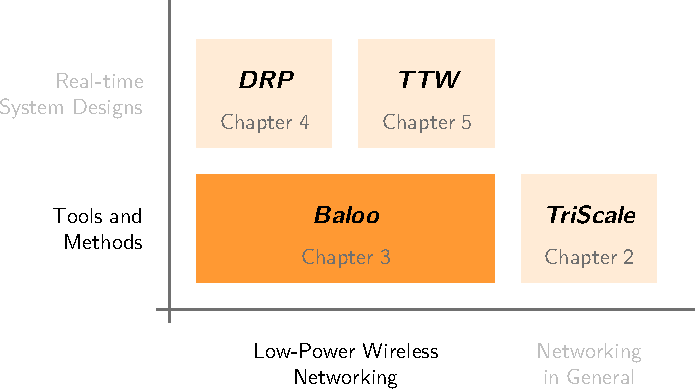
\includegraphics[scale=0.9]{chapter_baloo}
  \caption{Positioning of this chapter in the dissertation.
  \capt{This chapter presents \baloo, a design framework facilitating the implementation of low-power wireless networking protocols based on synchronous transmissions.}}
  \label{fig:chapter_baloo}
\end{figure}

% ------------------------------------------------------------------------------
% Claim
Thus, in this chapter, we study the feasibility of a design tool that would facilitate the development of network stacks based on \ST~(\cref{fig:chapter_baloo}); typically, such a tool would be useful for implementing our real-time protocol stacks (see \cref{ch:drp} and \cref{ch:ttw}).

\fakepar{Claim}
We propose and implement \baloo, a design framework for network stacks based on synchronous transmissions.
\baloo significantly lowers the entry barrier for harnessing the efficiency, reliability and mobility support of synchronous transmissions: users implement their protocol through a simple yet flexible API while \baloo handles all the complex low-level operations based on the users' inputs.

\baloo is flexible enough to implement a wide variety of network layer protocols, with only limited memory and energy overhead.

% ------------------------------------------------------------------------------
% Corresponding reference(s)
\begin{publi}

  The material from this chapter builds upon the work from Jonas Bächli~\cite{bachli2018Creating}. It relates to the following publication.

  \inlineRef{Synchronous Transmissions Made Easy: Design Your Network Stack with Baloo}{Romain Jacob, Jonas Bächli, Reto Da Forno, Lothar Thiele}{EWSN 2019. Beijung, China (February 2019)}

\end{publi}

% ------------------------------------------------------------------------------
% ------------------------------------------------------------------------------
% FORMER INTRO
% ------------------------------------------------------------------------------
% ------------------------------------------------------------------------------
% \newpage
% %Context
% \textsl{Synchronous Transmissions} (\ST) refers to a wireless communication technique that broadcast messages in a multi-hop network using flooding.
% This is made efficient by letting multiple transmitters send the \textsl{same packet} at the \textsl{same time}; henceforth the name of \emph{synchronous} transmissions.%
% \footnote{The name \textsl{concurrent transmissions} is also found in the literature.}
% \ST has been proven to be highly reliable and energy efficient, in particular for low-power wireless networks. Furthermore, flooding allows \ST to seamlessly support mobility by design.
% More informantion about \ST are presented in Introduction (\cref{ch:introduction}).
%
% %Problem
% Unfortunately, it is difficult to guarantee that multiple nodes actually send at the ``same time''.
% The required precision on synchronization depends \eg on the physical layer speed, the radio modulation speed or the encoding scheme.
% For typical low-power wireless motes available today, the synchronization must be in the order of \us for \ST to work reliably.
% Achieving such time synchronization requires to precisely control the timing of radio operations, which involves careful timer settings and interrupt handling.
% The integration of such ``low-level software'' within a entire network stack is challenging.
% Consequently, the adoption and development of \ST-based network stacks has been hindered by
% the lack of usable and flexible design tools.
%
% %Task and object
% Therefore, we developed \baloo: a flexible network stack design framework, designed to facilitate the development of protocols based on \ST. The key element of \baloo is a middleware layer which separates the radio management from the protocol implementation: \baloo provides a flexible application programming interface, while ensuring the correct timing of radio operations.
%
% %Findings
% \baloo is flexible enough to implement a wide variety of network layer protocols, with only limited memory and energy overhead.
% Most importantly \baloo makes \ST accessible: The software is open source and well documented.
% Since its development, \baloo has been used in a variety of projects, from both our team and external research groups.
% We believe that \baloo is an important enabler for a whole new class of Internet of Things applications leveraging the reliability, efficiency, and flexibility of \ST.

%
%
% This chapter presents \baloo, its design and the evaluation of its performance. We conclude with a brief description of projects that have been facilitated by \baloo, and finally discuss potential future developments, including standardization efforts.

% !TEX root =  ../00_thesis.tex

\section{Prolem Setting}
\label{sec:baloo_intro}

\squarepar{%
  Synchronous Transmissions (\ST) is an increasingly used wireless communication technology for low-power multi-hop networks. Popularized by Glossy~\cite{ferrari2011Glossy} in 2011, it has been proven to be highly reliable and energy efficient, as illustrated by the EWSN Dependability Competition ~\cite{schuss2017Competition}, where all wining solutions were based on \ST~\cite{escobar2018Competition,sommer2016Competition,lim2017Competition, escobar2019RedNodeBus, ma2019DeCoT} in the past four years (2016 to 2019).%
}

A \textsl{\ST primitive} refers to a protocol that efficiently realizes broadcast (\ie any-to-all communication) in bounded time, usually relying on \textsl{flooding}.
Flooding is a communication strategy that realizes broadcast by having all receivers of a packet retransmit this same packet to all their neighbours; the packet is thus ``flooded'' through the whole network. \ST makes flooding energy and time efficient by letting multiple wireless nodes transmit the packet \textsl{synchronously}, hence the name of \textsl{Synchronous Transmissions}. The successful reception of the packet can be achieved if the transmitters are tightly synchronized, thanks to \textsl{constructive interference} and the \textsl{capture effect}~\cite{yuan2013LetTalkTogether}.
The synchronization requirements vary from sub-\us to tens of \us, depending on the platform and modulation scheme~\cite{yuan2013LetTalkTogether}.
 %
%\footnote{Some background on flooding and \ST technology is provided in \cref{sec:baloo_overview}.}.
Such a broadcast primitive simplifies the design of network layer protocols: The underlying multi-hop network can be abstracted as a \textsl{virtual single-hop network} and thus be scheduled like a shared bus~\cite{ferrari2012LWB}.
One may refer to \cref{ch:introduction} for more details on \ST.

Since Glossy~\cite{ferrari2011Glossy}, many flavours of \ST primitives have been proposed to improve performance in terms of reliability, latency, and energy consumption.
To be more resilient to strong interference, Robust Flooding~\cite{lim2017Competition} is a primitive that modifies the RX-TX sequence from the original Glossy, whereas RedFixHop~\cite{escobar2016RedFixHop} uses hardware acknowledgements to minimize the number of retransmissions required.
Instead, some primitives aim to minimize latency for specific traffic patterns.
For example, Chaos~\cite{landsiedel2013Chaos} lets all nodes modify the packet being flooded to quickly aggregate information (\eg the max value of all sensor readings) or efficiently perform all-to-all data sharing to achieve distributed consensus~\cite{alnahas2017a2}.
Codecast~\cite{mohammad2018Codecast} also targets many-to-many exchange for a larger amount of data.
Pando~\cite{du2015Pando} is another primitive focused on high throughput, which uses fountain code and packet pipelining for efficient data dissemination.
Syncast~\cite{mohammad2017Improving} aims to reduce the radio on time required to save energy, while Less is More (LiM)~\cite{zhang2017LiM} is a primitive that reduces energy consumption using learning to avoid unnecessary retransmissions during flooding.

\squarepar{%
  All these primitives share the same drawback: Successful \ST requires low-level control of timers and radio events in order to meet \ST tight synchronization requirements (the order of \us).
  This degree of accuracy is difficult to achieve as it requires a detailed knowledge of the underlying hardware, low-level control of the radio operations, and a very careful management of software delays.%
}

As a result, designing a network stack based on \ST is a complex and time consuming task, for which only few solutions have been proposed.
One of the first was the Low-power Wireless Bus (LWB) ~\cite{ferrari2012LWB}, which tries to flexibly support all kinds of traffic patterns in a balanced trade-off between latency and energy consumption.
The same group designed eLWB~\cite{sutton2017eLWB}, a variation of LWB tailored to event-based data collection.
Sleeping Beauty~\cite{sarkar2016Sleeping} was later proposed to minimize energy consumption for data collection scenarios with many redundant sensor nodes.
Time-Triggered-Wireless (TTW -- \cref{ch:ttw})~\cite{jacob2017TTW_extended} was designed to minimize the end-to-end latency between communicating application tasks.
Finally, Crystal~\cite{istomin2018Interferenceresilient} has been proposed as a network stack specialized for sporadic data collection.
All these network stacks solely rely on Glossy as \ST primitive.
%
In principle however, the same protocol logic could benefit from \textsl{multiple} primitives. For example, an LWB network could use Robust Flooding~\cite{lim2017Competition} in case of high interference, then revert to Glossy~\cite{ferrari2011Glossy} for better time synchronization. If nodes need reprogramming, the software update can be quickly disseminated using Pando~\cite{du2015Pando}.
Designing a modular network stack supporting multiple \ST primitives adds a new level of complexity.

\begin{research_questions}
  \begin{description}
    \item[Question 1]
    Can we facilitate the design of wireless network stacks based on Synchronous Transmission?

    \item[Question 2]
    Can we implement flexible and adaptive protocols, potentially leveraging multiple \ST primitives, while guaranteeing that the timing requirements of \ST are met?
  \end{description}
\end{research_questions}

\fakepar{The problem}
To facilitate the network stack design (\question{1}),
a natural idea is to separate the concern of the timely execution of the primitives from the implementation of the protocol logic.
One way to achieve such separation of concerns is to use a \textsl{middleware} as part of the network stack.

%Challenges
The idea of a middleware for Wireless Sensor Networks (WSN) is not new, and the main challenge in such an endeavour is well-known.
As phrased by Mottola and Picco~\cite{mottola2012Middleware}, ``\textit{striking a balance between flexibility and complexity in providing access to low-level features is probably one of the toughest, yet most important, problems in WSN middleware}''.

The design of a middleware for \ST is particularly challenging.
Indeed, meeting the tight timing requirements for \ST is directly conflicting with the concept of abstraction of a middleware: How to guarantee that the network layer does not hinder the timing accuracy for \ST if it is itself unaware of the execution of the primitives? That is \question{2}.


\fakepar{The challenge} A middleware for \ST should meet the following requirements.
% This problem can be formulated by the following challenges:

\begin{features}

	\item[Usability]
	The middleware must realize a well-defined interface enabling runtime control from the network layer (which implements the protocol logic) over the execution of the underlying \ST primitives.

	\item[Generality]
	The middleware must enable the implementation of a large variety of network layer protocols.

	\item[Versatility]
	The middleware must enable one network layer protocol to use multiple \ST primitives and switch between them at runtime.

	\item[Synchronicity]
	The middleware must guarantee to respect the time synchronization requirements for \ST (from sub-\us to tens of \us~\cite{yuan2013LetTalkTogether}).
\end{features}

\pagebreak
%Task/Contibution
\fakepar{Our solution}
To address these challenges, we have designed \baloo, a flexible design framework for low-power network stacks based on \ST.%
\footnote{The framework provides the ``bare necessities'' for the design and implementation of \ST-based network stacks; so we called it \baloo.}
\baloo provides a large set of features enabling performant protocol designs, while abstracting away low-level hardware management such as interrupt handling and radio core control.
In summary:

\begin{itemize}
	\item
	We propose \baloo, a flexible design framework for low-power wireless network stacks based on \ST, illustrated in \cref{fig:stack_baloo}.

	\item
	We present the design of a middleware layer that meets all our requirements. This middleware forms the core component of \baloo.

	\item
	We showcase the usability of \baloo by re-implementing three well-known network stacks using \ST: the Low-power Wireless Bus (LWB)~\cite{ferrari2012LWB}, Sleeping Beauty~\cite{sarkar2016Sleeping}, and Crystal~\cite{istomin2018Interferenceresilient}.

	\item
	We illustrate the portability of \baloo by providing implementations for two platforms -- the CC430 SoC~\cite{CC430F6137} and the old but still heavily used TelosB mote~\cite{TelosB}.

	\item
	We demonstrate that \baloo induces only limited performance overhead (memory usage, radio duty cycle) compared to the original implementations.

\end{itemize}


\begin{figure}
  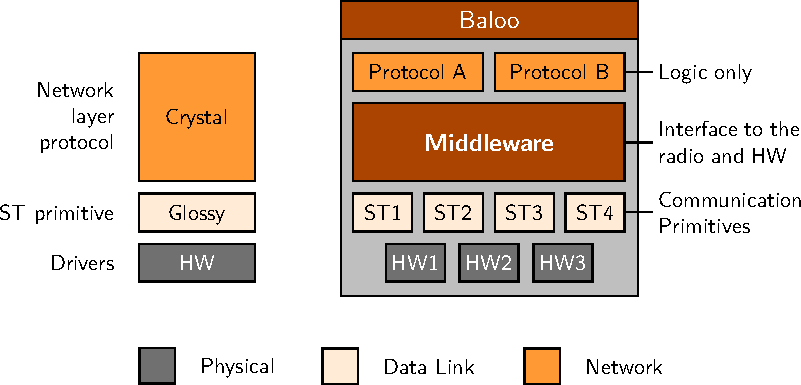
\includegraphics[scale=1]{stack_baloo.pdf}\\~\\
  \begin{minipage}[t]{.47\linewidth}
    \textbf{(a)} The implementation of the network layer protocol (Crystal) couples the interface to the underlying \ST primitive (Glossy) and the protocol logic, \ie how long are the communication rounds, which radio channel is used, \etc
  \end{minipage}
  \hfill
  \begin{minipage}[t]{.47\linewidth}
    \textbf{(b)} Thanks to its additional middleware layer, \baloo flexibly supports multiple \ST primitives and significantly reduces the efforts required to implement  network layer protocols compared to traditional stacks, like LWB~\cite{ferrari2012LWB} or Crystal~\cite{istomin2018Interferenceresilient}.
  \end{minipage}
  %
  \caption{Crystal~\cite{istomin2018Interferenceresilient} is a typical example of network stack based on \ST (\cref{fig:stack_baloo}a).
		Conversely, \baloo is a flexible design framework.
		It is based on a middleware layer that separates the concern of timely execution of \ST primitives from the implementation of the protocol logic (\cref{fig:stack_baloo}b).}
	\label{fig:stack_baloo}
\end{figure}

This chapter \emph{is not} meant to cover all details and inner mechanisms of \baloo, but mainly presents the core concepts of the framework.
\baloo is open source and the complete technical documentation is available online~(\cref{append:baloo_artifacts}).

% !TEX root = ../00_thesis.tex

\begin{figure}
	\centering
	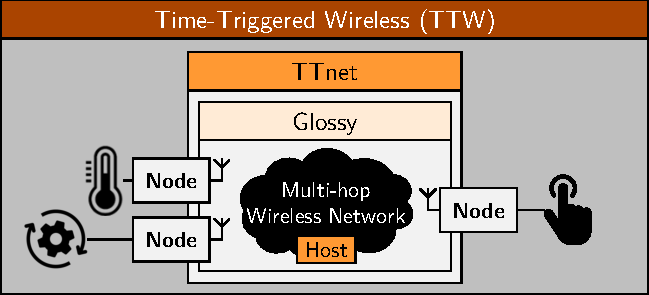
\includegraphics[scale=1]{ttw_overview}
	\caption{Overview of \TTW.
		\capt{Nodes execute distributed \CPS applications. They communicate over a multi-hop wireless network using Glossy floods~\cite{ferrari2011Glossy}.
		Communication is organized in \TTnet rounds~(\cref{fig:ttnet}) which are controlled by a central host (running on one of the nodes).
		\TTW is a global scheduler for the entire system: it co-schedules the execution time of all tasks and messages in order to reduce the end-to-end latency of applications and meet short deadlines.}
	}
	\label{fig:ttw_overview}
\end{figure}


% \caption{(a) General system model and (b) time-slotted execution of \TTW.
% \capt{%
% As in LWB\emph{~\cite{ferrari2012LWB}}, communication rounds are divided into time slots, in which Glossy floods are executed. Each color shows one flooding step.
% In \TTW, the first slot of each round contains a beacon sent by the host, followed by (up to) \nslotsmax slots, allocated to application messages. The beacons announce the identification number of the round (round \id) and trigger mode changes.
% }

\section{Overview of \TTW}
\label{sec:ttw_overview}

We first present \TTnet, a network stack based on synchronous transmissions (\ST), which serves as communication backbone for our solution~(\cref{subsec:ttnet}). We then introduce the concepts of \TTW~(\cref{subsec:ttw_concepts}), a system-wide scheduler built atop \TTnet to realize a wireless \CPS solution meeting the requirements described above.

\subsection{The \TTnet communication backbone}
\label{subsec:ttnet}

We consider a set of nodes connected by a wireless multi-hop network~(\cref{fig:ttw_overview}).
Each node is a low-power embedded device, typically battery-powered, with limited computational resources such as memory or processing power.
These devices collectively implement distributed applications (\eg closed-loop control). These applications are composed of multiple tasks and messages; the tasks are executed locally by the nodes; the messages are exchanged over the multi-hop wireless network.
In low-power wireless \CPS, a significant part of the energy is consumed by wireless communication. Thus, to minimize the energy consumption, we group messages into communication rounds, \ie time intervals where all nodes turn their radio on and communicate.
Each round is composed of dedicated time slots where nodes communicates using Glossy, a flooding protocol which delivers packets with a probability above 99.9\,\%~\cite{ferrari2011Glossy}.
The system is controlled centrally by a node called the host, which sends commands at the beginning of each round in a special slot called beacon.
Physically, one of the nodes plays the role of the host.
We call this network stack \TTnet~(\cref{fig:ttnet}).


\begin{figure}
	\centering
	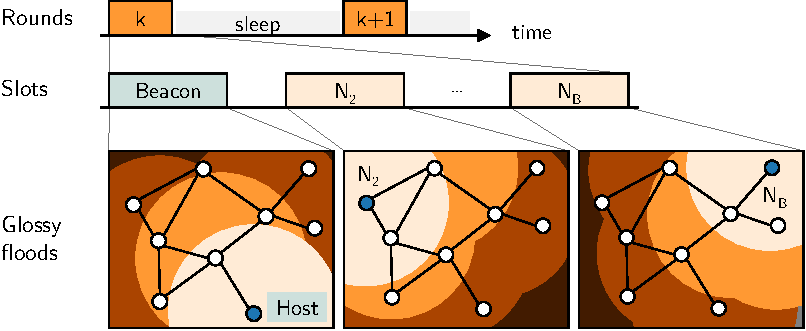
\includegraphics[scale=1]{ttnet}
	\caption{The \TTnet network stack.
	\capt{%
		\TTnet organizes communication in time-triggered rounds, between which nodes turn their radio off to save energy.
		The rounds are composed of (up to) \nslots communication slots preceded by a beacon, sent by the host to distribute runtime control information.
		In each slot, an one-to-all communication is realized using Glossy~\cite{ferrari2011Glossy}.}}
	\label{fig:ttnet}
\end{figure}

\TTnet concept of round-based communication using Glossy floods is inspired by the Low-power Wireless Bus (LWB)~\cite{ferrari2012LWB}; this design has several benefits:
\begin{itemize}

	\item
	It is based on Glossy, which has been proven to be highly reliable and energy efficient~(\cite{schuss2017Competition,lim2017Competition,escobar-molero2019Improving}).

	\item
	Glossy provides sub-microsecond time synchronization across the network~\cite{ferrari2011Glossy}, which is instrumental to achieve \feature{Timeliness} and \feature{Reliability}.

	\item
	The flooding process in Glossy is independent of the network state; thus it creates a virtual single-hop network where each node can communicate with every other node in bounded time. As a result, network stacks like LWB or \TTnet can be scheduled like a shared bus.

	\item
	As messages are flooded in the entire network, unicast multicast and broadcast are equivalent: for a given payload, the transmission time only depends on the network diameter (the maximal hop distance between nodes).

	\item
	Thanks to its stateless flooding logic, Glossy inherently supports \feature{Mobility}.

\end{itemize}

Despite these benefits, LWB or \TTnet alone cannot meet all the requirements of wireless \CPS. In particular, one must account for the scheduling of distributed tasks in order to provide end-to-end timing guarantees (\feature{Timeliness}).
\linebreak
This motivates the design of \TTW, a real-time scheduler for the \TTnet stack.

% ------------------------------------------------------------------------------
\subsection{Building-up \TTW}
\label{subsec:ttw_concepts}

The \TTnet is the communication backbone of \TTW.
Building on that structure, we design \TTW, a real-time scheduler for the entire wireless \CPS.

\TTW is based on four key concepts.

\begin{description}

	\item [Global co-scheduling]
	In order to minimize the achievable end-to-end latency, \TTW co-schedules the task executions and message transmissions, similarly to the state-of-the-art for wired protocols (\eg~\cite{craciunas2016Combined,zhang2014Task}).
	Moreover, the round-based design of \TTnet demands to integrates the communication rounds to the schedules. The allocation of messages to communication rounds is similar to a bin-packing problem~\cite{wikipedia2019BinPacking}.
	Combining pin-packing with traditional task-and-message co-scheduling approaches is non trivial~(\cref{sec:single_mode}).

	The resulting problem is a complex optimization that cannot be solved online, even less in a low-power setting.
	Therefore, \TTW statically synthesizes the schedule of all tasks, messages, and rounds to meet real-time constraints, minimize end-to-end latency, and minimize the energy consumed for communication.
	The schedule is synthesized by solving an MILP (mixed integer linear programming) formulation.

	\item[Static schedules]
	Since \TTW relies on static scheduling, we distribute the schedules at deployment time to limit the communication overhead at runtime, thus optimizing energy efficiency.
	Each node stores its own schedule information, thereby trading-off memory utilization with energy consumption; this significantly improves the \feature{Efficiency} of the system.



	\item[Multiple operation modes]
	The obvious drawback of using static schedules is that the system always execute the same schedule, compromising \feature{Adaptability}.
	\TTW mitigates this problem by using the traditional concept of operation modes~\cite{fohler1993changing}:
	Multiple schedules are computed offline and stored in the nodes' memory. The system can switch at runtime between different modes, thereby recovering some degree of \feature{Adaptability}.



	\item[Runtime control]
	At the beginning of each round, the host sends a beacon, which is used to control the system execution at runtime.
	A beacon contains the current round \id, the mode \id, and a trigger bit \SB used in the mode change procedure~(\cref{sec:modeChanges}).

	Thanks to the distributed schedule information, it is sufficient for any node to receive a single beacon to retrieve the system state (\ie the phase of the schedule given by the round \id) and therefore know
	% \begin{itemize}
		% \linebreak
		% \inlineitem
		(i)~which message to send in which slot, and
		% \\
		% \inlineitem
		(ii)~when to wake up for the next communication round.
		% \\
	% \end{itemize}
	If a node does not receive the beacon, it does not participate in the round. Hence, even if nodes miss some control information, they do not initiate a communication in a slot allocated to another node, thus guaranteeing conflict-free communication~(\feature{Reliability}).

\end{description}

By globally optimizing the entire system schedule, \TTW can meet tight end-to-end deadlines (tens of \ms) while minimizing the energy spent for wireless communication, thus addressing the \feature{Timeliness} and \feature{Efficiency} requirements.
The runtime control based on beacons provides \feature{Reliability}, while switching between multiple operation modes at runtime offers some degree of \feature{Adaptability}.
Finally, \feature{Mobility} is supported by design thanks to the stateless logic of Glossy~\cite{ferrari2011Glossy}, the underlying communication primitive used by \TTW.

\begin{remark}
	\TTW combines offline scheduling and online decisions whereas \DRP~(\cref{ch:drp}), by contrast, does everything online.
	Hence, \TTW trades the flexibility of execution of the distributed application tasks for short latency and fast mode changes.
\end{remark}

% !TEX root = ../00_thesis.tex

\section{System Model and Scheduling Problem}
\label{sec:model}

\fakepar{Nodes}
We denote by \nodeset the set of \emph{nodes} in the system.
Nodes implement distributed applications, composed of multiple tasks to execute and  messages to exchange.
A node is considered capable of performing one task execution and one message transmission simultaneously; this is supported by state-of-the-art wireless \cps platforms featuring two cores, such as the NXP LPC541XX~\cite{nxpLPC541XX}, VF3xxR~\cite{nxpVF3xxR}, or more generally any platform following the Dual-Processor Platform concept~(\cref{sec:dpp}).

\fakepar{Applications}
We denote by \appset the set of \emph{applications} in the system.
Each distributed application is composed of \emph{tasks} and \emph{messages} connected by precedence constraints described by a directed acyclic graph, where vertices and edges represent tasks and messages, respectively. We denote by \app.\predG the \emph{precedence graph} of application \app~(\cref{fig:precedence_graph}).
Each application executes at a periodic interval $\app.p$, called the \emph{period}.
An application execution is completed when all tasks in \predG have been executed.
All tasks and messages in \app.\predG share the same period, $\app.p$.
Applications are subject to real-time constraints: The application \emph{relative deadline}, denoted by $\app.d$ represents the maximum tolerable \emph{end-to-end delay} to complete the execution. The deadline is arbitrary (\ie it has no relation with the period $\app.p$).
Certain critical applications may require to keep the same schedule (\eg same task offsets) when switching between operation modes.
We call these \emph{persistent applications} and denote their set by \persappset; $\persappset \subset \appset$.
In summary, an application \app is characterized by

\pagebreak

\begin{align*}
\app \; = \; \{ \quad
	 \app.p
	\quad &\text{--\quad period} \\
	 \app.d
	\quad &\text{--\quad end-to-end deadline} \\
	 \app.\predG
	\quad &\text{--\quad precedence graph} \quad\quad \}
\end{align*}

\fakepar{Tasks}
We denote by \taskset the set of tasks.
A node executes at most one task at any point in time and we consider non-preemptive task scheduling.
Each task $\tau$ is mapped to a given node $\tau.map$, on which it executes within a WCET (worst-case execution time) $\tau.e$.
The \emph{task offset} $\tau.o$ represents the start of the task execution, relative to the beginning of the application execution.
A task can have an arbitrary number of preceding messages, \ie messages that must be received before the task can start. $\tau.prec$ denotes the set of preceding message \ids.
Within one application, each task is unique; however, the same task may belong to multiple applications (\eg the same sensing task may source different feedback loops). If so, we consider that these applications have the same period.
In summary, a task $\tau$ is characterized by
\begin{align*}
\tau \; = \; \{ \quad
	 \tau.o
	\quad &\text{--\quad offset} \\
	 \tau.\map
	\quad &\text{--\quad mapping} \\
	 \tau.e
	\quad &\text{--\quad WCET} \\
	 \tau.\prec
	\quad &\text{--\quad preceding message set} \\
	 \tau.p
	\quad &\text{--\quad period (equal to $\app.p$)} \quad \quad \}
\end{align*}

\fakepar{Messages}
We denote by \messageset the set of messages.
Every message $m$ has at least one preceding task, \ie a task that needs to finish before the message can be transmitted. The set of preceding task \ids is denoted by $m.prec$.
% All preceding tasks must be mapped to the same node.
The \emph{message offset} $m.o$, relative to the beginning of the application execution, represents the earliest time the message $m$ can be allocated to a round for transmission, \ie after all preceding tasks are completed.
The \emph{message deadline} $m.d$, relative to the message offset, represents the latest time when the message transmission must be completed, \ie the earliest offset of successor tasks.
All messages share the same maximal payload \Lmax.
Messages are not necessarily unique, \ie multiple edges of \app.\predG can be labeled with the same message $m$, which captures the case of multicast or broadcast~(\cref{fig:precedence_graph}).
If the same message belongs to multiple applications, we consider that these applications have the same period.
In summary, a message $m$ is characterized by
\begin{align*}
m \; = \; \{ \quad
	 m.o
	\quad &\text{--\quad offset} \\
	 m.d
	\quad &\text{--\quad deadline} \\
	 m.\prec
	\quad &\text{--\quad preceding task set} \\
	 m.p
	\quad &\text{--\quad period (equal to $\app.p$)} \quad \quad \}
\end{align*}


\begin{figure}
\centering
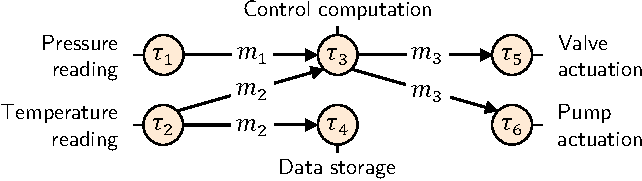
\includegraphics[scale=1]{precedence_graph}
\caption{An example application and its precedence graph \predG.
\capt{The execution starts with sensor readings -- either $\tau_1$ or $\tau_2$. After both have been received by the controller, actuation values are computed ($\tau_3$), multicast to the actuators ($m_3$), and applied ($\tau_5$ and $\tau_6$).
%All tasks must be completed before the application end-to-end deadline $\app.d$.
}}
\label{fig:precedence_graph}
\end{figure}

\pagebreak

\fakepar{Operation modes}
We denote by \modeset the set of operation modes (also simply called ``modes'').
These modes represent mutually exclusive phases of the system, \eg boostrapping, normal, and emergency modes; each having its own schedule.
Each mode has a unique \emph{priority} \modeany.\prio, used for scheduling purposes~(\cref{sec:multi_mode}).
A mode \modeany is characterized by
\begin{align*}
\modeany \; = \; \{ \quad
	 \appi\, , \;
	 \appj\, , \; \ldots
	\quad &\text{--\quad applications to execute}\\
	 \modeany.\prio
	\quad &\text{--\quad priority} \quad \}
\end{align*}
We write $\app \in \modeany$ to denote that \app is executing in mode \modeany.
When unambiguous, we use \modeany to denote the set of applications executing in mode \modeany.
The mode \emph{hyperperiod} \modeHyperperiod is the least common multiple of the mode's applications.
Possible transitions between modes at runtime are described with the \emph{mode graph} \modeGraph~(\cref{fig:modeGraph}). The mode graph is undirected; a transition from \modei to \modej implies that it is possible to transition from \modej to \modei as well.



\fakepar{Rounds}
The schedule of a mode \mode{} contains $R_{\mode{}}$ \emph{communication rounds} $r$.
Rounds are \emph{atomic}; that is, they cannot be interrupted. Therefore, the ordering of messages within one round does not matter.%
%
\footnote{\TTW could be extended to account for the relative ordering of messages in a round. In theory, this would allow to further reduce the achievable latency of applications at the cost of a more complex synthesis problem to solve.}
%
Each round $r$ is composed of \nslotsround slots (with a maximum of \nslotsmax), each allocated to a unique message $m$.
This results in a round length $\Tround = \Toffset + \nslotsround*\Tslot$, where \Tslot is the length of one communication slot, and \Toffset is the constant time overhead per round.
The round \emph{starting time} $r.t$ is the start of the round relative to the beginning of the mode hyperperiod.
The \emph{allocation vector} $r.[\nslotsround]$ is a vector of size \nslotsround containing the \ids of the messages allocated to the slots. $r.B_s$ denotes the allocation of the $s$-th slot.
In summary, a round $r$ is characterized by
\begin{align*}
r \; = \; \{ \quad
	 r.t
	\quad &\text{--\quad starting time} \\
	 r.[B]
	\quad &\text{--\quad allocation vector}  \quad \}
\end{align*}


\fakepar{Scheduling problem}
We consider that all modes, applications, task mappings and WCETs are given. For a given mode \mode{}, the remaining variables define the mode schedule, denoted by \sched{\mode{}}:
\begin{align*}
&\sched{\mode{}} \, = \,
	\left\lbrace
	\begin{tabular}{c|l}
	$\tau.o, \, m.o, \, m.d$
	&
	$\forall \; \app \in \mode{}, \;
	(\tau,m) \in \app.\predG$
	\\
	$r_k.t, \, r_k.[\nslotsmax]$
	&
	$\forall \; k \in [1, \, R_{\mode{}}]$
	\end{tabular}
	\right\rbrace
\end{align*}

A schedule for mode \modeany is said to be \emph{valid} if all applications executing in \modeany meet their end-to-end deadlines.
The scheduling problem to solve consists in deriving valid schedules for all operation modes in \modeset such that
\begin{description}
	\item [\objective{1}]
	The number of communication rounds is minimized, thereby minimizing the energy consumed for wireless communication.
	\item [\objective{2}]
	All persistent applications $\persappset \subset \appset$ seamlessly switch between modes; \ie their schedule remains the same over a mode change.
\end{description}

All inputs and output of the problem are summarized in \cref{table:ttw_inputs_outputs}.

\begin{table}
	\caption{Inputs and outputs of the scheduling problem solved by \TTW}
	\label{table:ttw_inputs_outputs}
	\smaller{\input{\ChapPath/Tables/in_out.csv}}
\end{table}

\fakepar{Application use case}
Consider the control of physical systems demanding update rates in the order of tens of \ms, which are common in an industrial context~\cite{akerberg2011Future}.
The classical proof-of-concept application is the closed-loop control of an inverted pendulum~\cite{boubaker2012inverted}.
With \TTW, one can use low-power wireless technology to remotely control multiple such pendulums, as demonstrated in~\cite{mager2019Feedback}.
Different \TTW operation modes may correspond to different control tasks: \eg solely stabilizing the pendulums or synchronizing their positions~\cite{mager2019Demo}.
Furthermore, thanks to the stateless logic of \TTnet (inherited from Glossy~\cite{ferrari2011Glossy}), \TTW inherently supports \feature{Mobility}.%
%
\footnote{Mobility experiment (1min): \href{https://youtu.be/19xPHjnobkY}{youtu.be/19xPHjnobkY}}

\pagebreak

\fakepar{Roadmap}
The rest of this chapter presents how \TTW solves the scheduling problem described above.
In \cref{sec:single_mode}, we present how to synthesize a valid schedule for a single mode such that the number of communication round used is minimized~\objective{1}.
Then, in \cref{sec:multi_mode}, we address the extension to the multi-mode case, and in particular how to allow applications to keep the same schedules in different modes~\objective{2}.
The subsequent sections discuss our implementation of \TTW and its performance evaluation.

% !TEX root = ../00_thesis.tex

% ------------------------------------------------------------------------------
\section{Single Mode Schedule Synthesis}
\label{sec:single_mode}
% ------------------------------------------------------------------------------
\squarepar{%}
	\TTW statically synthesizes the schedule of all tasks, messages, and communication rounds to meet real-time constraints by solving a MILP formulation.
	This section presents how to solve it efficiently and ensure that the resulting schedule minimizes the number of communication rounds~\objective{1}.

	The schedule of a mode \modeany is computed for one hyperperiod, after which it repeats itself.
	To minimize the number of rounds used while handling computational complexity, we solve the problem sequentially, as described in~\cref{alg:outerlayer}.
	Each formulation considers a fixed number of rounds $R_{\mode{}}$ to be scheduled, starting with $R_{\mode{}}=0$. The number of rounds is incremented until a feasible solution is found, or until the maximum number of rounds $R_{max}$ (the number of rounds that can ``fit'' into one hyperperiod) is reached.
	Thus, \cref{alg:outerlayer} guarantees by construction that if the problem is feasible, the synthesized schedule is optimal in terms of number of rounds used.%
}

\begin{algorithm}
\begin{algorithmic}
\smaller
\Require
	mode \mode{},\;
	$\app \in \mode{}$,\;
	$\tau.\map$,\;
	$\tau.e$, \;
	\nslotsmax, \;
	\Toffset
\Ensure
	\sched{M}

\State $LCM \gets$ \textit{hyperperiod}(\mode{})
\State $R_{max} \gets floor(LCM/\Toffset)$
\State $R_{\mode{}} \gets 0$

\While{$R_{\mode{}} \leq R_{max}$}
	\State formulate the MILP for mode \mode{} using $R_{\mode{}}$ rounds
	\State [ \sched{M}, \textit{feasible} ] = \textit{solve}( MILP )
	\If {\textit{feasible}}
		\Return \sched{M}
	\EndIf
	\State $R_{\mode{}} \gets R_{\mode{}}+1$
\EndWhile
\State \Return 'Problem infeasible'
\end{algorithmic}
\caption{\small Pseudo-code of the single-mode schedule synthesis}
\label{alg:outerlayer}
\end{algorithm}

The MILP formulation contains a set of classical scheduling constraints:
% \begin{itemize}
%
% 	\item
	The precedence constraints between tasks and messages must be respected;
	%
	% \item
	Applications end-to-end deadlines must be satisfied;
	%
	% \item
	Nodes process at most one task simultaneously;
	%
	% \item
	Communication rounds must not overlap;
	%
	% \item
	Rounds must not be allocated more then \nslotsmax messages.
%
% \end{itemize}
	These constraints can be easily formulated using our system model (full formulation in \cref{appendix:ttw_artifacts}).
	However, one must also guarantee that the allocation of messages to rounds is valid, \ie
	\begin{description}
		\squarepar{%}
			\item [\constraint{1}]
			Messages must be served in rounds that start after their release time.%
			\item [\constraint{2}]
			Messages must be served in rounds that finish before their deadline.%
		}
	\end{description}%
In other word, we must integrate the bin-packing problem of messages to rounds within the MILP formulation.
This is non-trivial and a major difference with the existing approaches for wired architectures~(\eg \cite{craciunas2016Combined}).

To address this challenge, we first formulate the constraints \constraint{1} and \constraint{2} using \emph{arrival}, \emph{demand}, and \emph{service} functions, \af \df and \sf, using network calculus~\cite{leboudec2001Network}.
Those functions count the number of message instances released, with passed deadlines, and served since the beginning of the hyperperiod, respectively.
These functions are illustrated in \cref{fig:afdfsf}.
It must hold that
\begin{flalign}
\label{eq:df<sf<af}
&\forall\, m_i \in \messageset, \;\forall\, t,
&&\df_i(t) \leq \sf_i(t) \leq \af_i(t)
&&\\
\label{eq:af_def}
&\text{with},
&&\af_i: \; t \;
	\longmapsto \; \left \lfloor{\frac{t-m_i.o}{m_i.p}}\right \rfloor 	+ 1
	&&\\
\label{eq:df_def}
&\text{and},
&&\df_i: \; t \;
	\longmapsto \; \left \lceil{\frac{t-m_i.o-m_i.d}{m_i.p}}\right \rceil
	&&
\end{flalign}

However, as the service function stays constant between the rounds, we can formulate \constraint{1} and \constraint{2} as follows\\
$\forall\, m_i \in \messageset, \; \forall\, j \in [1 .. R_{\mode{}}], $
\begin{flalign}
\label{eq:af_const}
&\textup{\constraint{1}} \quad  : \quad
	&\sf_i(r_j.t + \Tround) \, &\leq \, \af_i(r_j.t)
	&&
\\
\label{eq:df_const}
&\textup{\constraint{2}} \quad  : \quad
	&\sf_i(r_j.t)  \, &\geq \, \df_i(r_j.t + \Tround)
	&&
\end{flalign}

\begin{figure}
\centering
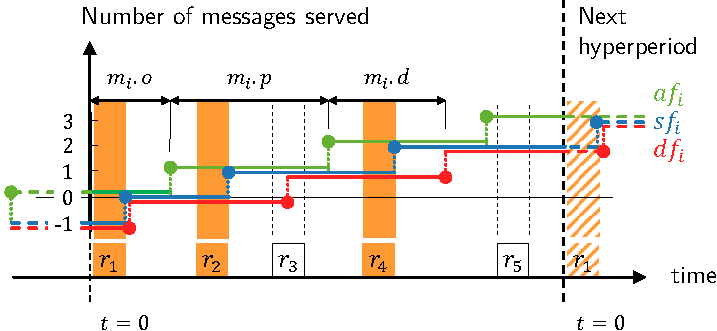
\includegraphics[scale=1]{afdfsf}
\caption{Representation of arrival, demand, and service functions of message $m_i$.
The lower part shows the five round, $r_1$ to $r_5$, scheduled for the hyperperiod.
\capt{%
$m_i$ is allocated a slot in the colored rounds, \ie $r_1$, $r_2$, and $r_4$.
The allocation of $m_i$ to $r_3$ instead of $r_2$ would be invalid, as $r_3$ does not finish before the message deadline, \ie it violates \constraint{2}.
However, the allocation of $m_i$ to $r_5$ instead of $r_1$ would be valid and result in $r_0.B_i = 0$.}
}
\label{fig:afdfsf}
\end{figure}


The arrival and demand functions are step functions. They cannot be used directly in an MILP formulation, however
\begin{flalign}
\label{eq:af=k}
&\forall \; k \in \mathbb{N}, \quad
&&\af_i(t) = k
	\quad \Leftrightarrow \quad
	0 \, \leq \, t - m_i.o - (k-1)m_i.p \,<\, m_i.p &&\\
&\text{and} %\hspace{30pt}
&&\df_i(t) = k
\label{eq:df=k}
	\quad \Leftrightarrow \quad
	0 \, < \, t - m_i.o - m_i.d - (k-1)m_i.p \,\leq\, m_i.p &&
\end{flalign}

For each message $m_i\in \messageset$ and each round $r_j$, $j \in [1..R_{\mode{}}]$, we introduce two integer variables $k^a_{ij}$ and $k^d_{ij}$ that we constraint to take the values of \af and \df at the time points of interest (respectively $r_j.t$ and $r_j.t + \Troundj$). That is,
\begin{align}
\label{eq:ka} %\qquad
0 \, \leq \, r_j.t
	&-m_i.o - (k^a_{ij}-1)m_i.p \,<\, m_i.p\\
\label{eq:kd} %\qquad
0 \, < \, r_j.t
	&+\Troundj - m_i.o - m_i.d - (k^d_{ij}-1)m_i.p \,\leq\, m_i.p\\
\notag
\text{Thus,} \hspace{15pt} &\eqref{eq:ka} \quad \Leftrightarrow  \quad
	 \af_i(r_j.t) = k^a_{ij} \\
\notag
	&\eqref{eq:kd} \quad \Leftrightarrow \quad
	\df_i(r_j.t + \Troundj) = k^d_{ij}
\end{align}

Finally, we must express the service function \sf, which counts the number of message instances served \emph{at the end} of each round.
Remember that $r_k.B_s$ denotes the allocation of the $s$-{th} slot of $r_k$ (\ie the $id$ of the message allocated to the slot).
For any time $t \in \; [ \; r_{j}.t + \Troundj \, ; \,  r_{j+1}.t + \Troundj \; [$, the number of instances of message $m_i$ served is
\begin{align*}
	\sum_{\substack{k = 1}}^{j} \;\;
	\sum_{\substack{s = 1}}^{B}
	 \; r_k.B_s
	 \quad s.t. \; B_s = i
\end{align*}

It may be that $m.o + m.d > m.p$, resulting in $\df(0)=-1$ (\cref{eq:df_def}), like it is the case in \cref{fig:afdfsf}. This ``means'' that a message released at the each of one hyperperiod will have its deadline in the \emph{next} hyperperiod.
To account for this situation, we introduce, for each message $m_i$, a variable $r_0.B_i$ set to the number of such ``leftover'' message instances at $t=0$. Finally, for each message $m_i \in \messageset$, and  $t \in \; [ \; r_{j}.t + \Troundj \, ; \,  r_{j+1}.t + \Troundj \; [$,
\begin{flalign}
\label{eq:sf_def}
\sf_i: \; t \;
	&\longmapsto \;
	\sum_{\substack{k = 1 \\[2pt]s.t. \; r_k.t + \Troundk \, < \, t}}^{j}\;\;
	\sum_{\substack{s = 1 \\[2pt]s.t. \; B_s = i}}^{B}
	 r_k.B_s - r_0.B_i
\end{flalign}

Ultimately, \constraint{1} and \constraint{2} can be formulated as MILP constraints using \cref{eq:ka,eq:kd}, and the following two equations:
\begin{align}
&
\eqref{eq:af_const}\quad	 \Leftrightarrow
	\quad
	\sum_{k = 1}^j
	\sum_{\substack{s = 1 \\[2pt]s.t. \; B_s = i}}^{B}
	 \; r_k.B_s - r_0.B_i \; \leq\;  k^a_{ij}
\\
&
\eqref{eq:df_const}\quad	 \Leftrightarrow
	\quad
	\sum_{k = 1}^{j-1}
	\sum_{\substack{s = 1 \\[2pt]s.t. \; B_s = i}}^{B} \; r_k.B_s - r_0.B_i
	\; \geq\;
	k^d_{ij}
\end{align}


\fakepar{Objective function}
Within our scheduling framework, the MILP does not need to optimize any objective function. Indeed, we mainly want to minimize of the number of rounds $R$ used in the schedule, which is achieved by incrementally increasing the number of rounds until a valid schedule is found~(\cref{alg:outerlayer}).

However, when considering the multi-mode case~(\cref{sec:multi_mode}), it is beneficial to maximize the message deadlines, as illustrated in \cref{fig:msg_deadline_maximization}.
In a nutshell, it relaxes the constraints that are inherited between different modes, and therefore improve the schedulability of the whole problem.
Concretely, the deadline maximization is achieved by setting the following objective to the MILP solver
\begin{align}
&obj \; = \; \sum_{m_i\in \messageset} \, m_i.d
\end{align}


\begin{figure}
	\begin{subfigure}[t]{.48\linewidth}
	\centering
	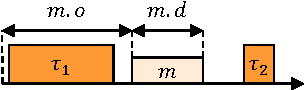
\includegraphics[scale=1]{msg_deadline_base}
	\caption{%
	Example schedule without deadline maximization.
	}
	\label{subfig:msg_deadline_base}
	\end{subfigure}%
	\hfill
	\begin{subfigure}[t]{.48\linewidth}
	\centering
	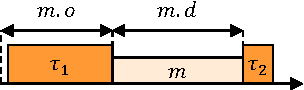
\includegraphics[scale=1]{msg_deadline_maximized}
	\caption{%
	Example schedule with deadline maximization}
	\label{subfig:msg_deadline_maximized}
	\end{subfigure}
	\caption{Illustration of the impact of the message deadlines maximization.
	\capt{%
		If~\cref{subfig:msg_deadline_base} is a valid schedule, then \cref{subfig:msg_deadline_maximized} is also valid, but it
		relaxes the constraints on other modes which also contain message $m$.
		Maximizing the message deadlines improves the schedulability of the multi-mode problem~(\cref{sec:multi_mode}).
	}}
	\label{fig:msg_deadline_maximization}
\end{figure}

% !TEX root = ../00_thesis.tex

% ------------------------------------------------------------------------------
\section{Synthesis of Compatible Multi-Mode Schedules}
\label{sec:multi_mode}
% ------------------------------------------------------------------------------


\TTW statically co-schedules all tasks and messages in order to satisfy tight deadline constraints~(\cref{sec:single_mode}).
To preserve a certain degree of adaptability at runtime, we support multiple operation modes.
Doing so requires to ensure predictable mode switches; that is, applications always meet their end-to-end deadlines~\objA and the persistent applications have compatible schedules in different modes~\objB.

% \TODO{needed?}
% We will formulate this schedule compatible with a continuity constraint~(\cref{def:continuity_constraint}). When the mode schedules are compatible, we say that the modes are \emph{conflict-free}.

The multi-mode case is essentially a multi-objective problem. One could decide to minimize the overall number of rounds used (\ie the sum of rounds in all the modes); however, it might also be interesting to optimize the ``most common mode''; this is, the mode in which the system operates most of the time.
Ultimately, one must weight the different modes to define a globally optimal solution.

\squarepar{%}
	Instead of solving the entire multi-mode problem at once, which would have scalability issues, we solve the problem sequentially: one mode at a time, in order of increasing priority.
	However, ensuring schedule compatibility between the different modes~\objective{2} creates dependencies, as illustrated below.%
}

\begin{example}
\label{exp:sched_conflict_basic}
	Let us consider the mode graph in \cref{fig:modeGraph} and assume that all applications are persistent.
	The modes are scheduled sequentially, starting with the highest-priority mode \mode{1}, which is freely scheduled.
	When mode \mode{2} is scheduled, the schedule for application \appl{2} is inherited from mode \mode{1}~\objective{2} and the schedules for applications \appl{3} and \appl{4} are synthesized without constraints.
	In \mode{3}, the specified applications, \appl{5} and \appl{6}, are new and can be scheduled without constraints.
	Then, in mode \mode{4}, the specified applications, \appl{1} and \appl{5}, have both been previously scheduled and thus must be inherited~\objective{2}.
	However, as mode \mode{3} has been scheduled without constraint, the schedule synthesized for \appl{5} may be non-compatible with that of \appl{1} from mode \mode{1}. This leads to a conflict in \mode{4} and thus renders the sequential synthesis of the multi-mode problem unfeasible~(illustrated in \cref{fig:example_sched}).
\end{example}

\begin{figure}
\centering
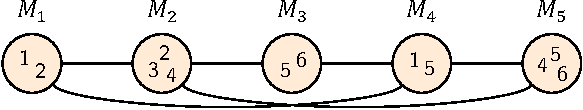
\includegraphics[scale=1]{modeGraph}
\caption{The mode graph \modeGraph discussed in \cref{exp:sched_conflict_basic,exp:sched_domain}.
\capt{Five modes are represented by circles, the possible transitions between modes as arcs. Six applications \appl{1} to \appl{6} are specified. The specification is shown with the numbers in the circles; \eg $S_1 = \{\appl{1},\appl{2}\}$. Mode \modei has priority $i$.}}
\label{fig:modeGraph}
\end{figure}

\begin{figure}
	\begin{subfigure}[t]{.48\linewidth}
		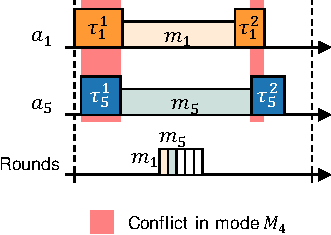
\includegraphics[scale=1]{example_sched_conflict}
		\caption{%
		\appl{5} is scheduled in mode \mode{3} without considering the previously computed schedule of \appl{1}, which leads to a conflict in mode \mode{4}.}
		\label{subfig:example_sched_conflict}
	\end{subfigure}%
	\hfill
	\begin{subfigure}[t]{.48\linewidth}
		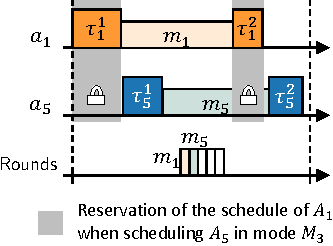
\includegraphics[scale=1]{example_sched_reservation}
		\caption{%
		\appl{5} is scheduled in mode \mode{3} considering the schedule of \appl{1} as \emph{reserved}. Thus, a compatible schedule for \appl{5} is computed, which prevents conflicts due to schedule inheritance in mode \mode{4}.}
		\label{subfig:example_sched_reservation}
	\end{subfigure}
	\caption{%
		Representations of the schedule of applications \appl{1} and \appl{5} from~\cref{exp:sched_conflict_basic}.
		For the sake of illustration, we consider that all tasks are mapped to the same node.
		\appl{1} and \appl{5} are scheduled respectively in mode \mode{1} and \mode{3}, and must both be inherited in mode \mode{4}.
		In~\cref{subfig:example_sched_conflict}, overlapping task schedules result in a conflict, while in~\cref{subfig:example_sched_reservation}, it was prevented by reserving \appl{1}'s schedule.
		The situation is different for the messages: overlapping message schedules is no issue, it simply represents a time interval where both messages can be served during the same round, as shown in this example.
	}
	\label{fig:example_sched}
\end{figure}

As illustrated in~\cref{exp:sched_conflict_basic}, it may be necessary to ``reserve the space'' of previously scheduled applications (\ie in previous modes) in order to avoid schedule conflicts.
The simplest approach is to reserve the space of \emph{all previous scheduled applications}. This is definitely safe but often pessimistic, as there may not be risk of conflicts for certain applications.

In this section, we derive the set of schedule reservations that is necessary and sufficient to prevent inheritance conflicts.
We first formalize the continuity constraints that we want to satisfy~\objB~(\cref{subsec:continuity_constraints}).
Then, we characterize conflicting modes and formalize how continuity constraints may lead to conflicts~(\cref{subsec:conflict_def}).
Finally, we derive the minimally restrictive reservations that are necessary and sufficient to prevent conflicts while satisfying \objB~(\cref{subsec:min_constraints}).

% ------------------------------------------------------------------------------
%	a.	Application domain decomposition -> Real-time apps to be preserved across diff modes
\subsection{Continuity Constraints}
\label{subsec:continuity_constraints}

The schedule synthesis returns the application schedules, \ie the task and message offsets and the message deadlines; and the round schedules, \ie the round starting times and the allocation vector.
We abstract an application schedule with a scheduling function $s$ as follows.

\begin{definition}[Scheduling function]
\label{def:sched_funtion}
The scheduling function $s$ is defined over the set of applications \appset and returns, for a given application \app, all the parameters characterizing the schedule of application \app. The schedule of an application \app is denoted by $s(\app)$.
The scheduling function is extended to sets of applications as follows.
\begin{equation*}
\forall \, S \subset \appset \; , \quad s(S) = \bigcup_{\app\in S} s(\app)
\end{equation*}
$s_\mode{}(\app)$ denotes the schedule of application \app in mode \modeany.
\end{definition}

All persistent applications $\app \in \persappset$ are subject to continuity constraints,  formalized as follows.
\begin{definition}[Continuity constraint]
\label{def:continuity_constraint}
\begin{align}
\intertext{$\forall\, \app \in \persappset, \; \forall\, (\modei, \modej) \in \modeset^2,$}
& \app \in \modei \; \wedge \; \app \in \modej \; \wedge \; \modeGraph(\modei,\modej) = 1
	\quad \Rightarrow \quad
	s_\modei(\app) = s_\modej(\app)
\end{align}
In other words, an executing application must keep the same schedule, regardless of mode changes.
\end{definition}


\begin{definition}[Schedule domains]
\label{def:sched_domains}
The schedule domains of an application are the (possibly multiple) subsets of modes in which the application schedule must remain the same.
\end{definition}

\begin{corollary}
	%Non real-time applications have schedule domains of size 1.
	Two modes \modei and \modej belong to the same schedule domain of an application $\app \in \persappset$ if and only if
	\begin{itemize}
		% \item $\app \in \persappset$,
		\item \app is scheduled in both modes, \ie $\app \in \modei \; \wedge \; \app \in \modej$, and
		\item There is a possible transition between the two modes, \ie $\modeGraph(\modei, \modej) = 1$.
	\end{itemize}
\end{corollary}

\proof
Multiple modes belong to the same schedule domain because of a continuity constraint.
The formalization of the schedule domains directly follows from~\cref{def:continuity_constraint}
\qed

The mode graph can be analyzed to extract the schedule domains of any application.
A simple approach entails considering the sub-graph \modeGraphA from \modeGraph, \ie where one keeps only the modes in which application \app is specified.
Every connected component of \modeGraphA is a schedule domain of \app.

\begin{hypothesis}
	\label{hyp:single_domain}
	We consider in the rest of this chapter that (i)~all applications are persistent, and (ii)~applications have a single scheduling domain.
\end{hypothesis}

\cref{hyp:single_domain} induces no loss of generality. Indeed, non-persistent applications present in multiple modes can be replaced by distinct applications, with the same parameters, executing in one mode each.
Similarly, persistent applications different scheduling domains can be replicated into different applications having one domain each.
This is illustrated in the following example.

\begin{example}\label{exp:sched_domain}
Consider again the mode graph in \cref{fig:modeGraph}. Application \appl{6} has two distinct application domains, $\{\mode{3}\}$ and $\{\mode{5}\}$, which can be modeled as two distinct applications \appl{6.3} and \appl{6.6} executing in \mode{3} and \mode{6} respectively.

On the contrary, \appl{1} has only one schedule domain, $\{\mode{1},\mode{4}\}$.
If \appl{1} is not persistent, the continuity constraint does not apply~(\cref{def:continuity_constraint}).
Thus, \appl{1} can be equivalently modeled as two distinct applications \appl{1.1} and \appl{1.4} executing in \mode{1} and \mode{4} respectively.
\end{example}


% ------------------------------------------------------------------------------
\subsection{Characterization of Conflicts}
\label{subsec:conflict_def}

\squarepar{%}
	As illustrated in \cref{exp:sched_conflict_basic}, the continuity constraint may lead to conflicts, leading to the failure of the multi-mode schedule synthesis problem, while a solution could exist.
	In particular, if a given mode \mode{} belongs to the schedule domains of two different applications which have been independently scheduled in higher priority modes, there is a risk of conflict, \ie the two inherited schedules may be non-compatible.
	This section formalizes the notions of (virtual) legacies and conflicting modes.
	$\overline{X}$ denotes the complement of $X$; \ie $\overline{X} = \appset \setminus X$.
	For each mode \modei, we define four sets of applications.%
}

\textbf{Known applications} are the applications previously scheduled in higher priority modes. The set of known applications of mode \modei is denoted \knownAppi:
	\begin{equation}
	\knownAppi = \cup_{j = 1}^{i-1} \; \modej
	\end{equation}

\textbf{Free applications} are the newly scheduled applications in mode \modei, \ie no higher priority mode belongs to the schedule domain of these applications.
	The set of free applications of mode \modei is denoted \freeAppi :
	\begin{equation}
	\freeAppi = \modei \; \cap \; (\appset \setminus \knownAppi) = \modei \; \cap \; \overline{\knownAppi}
	\end{equation}

\textbf{Legacy applications} are the applications previously scheduled in higher priority modes which must be scheduled in mode \modei.
	Since we assume a single scheduling domain~(\cref{hyp:single_domain}), \modei necessarily belongs to the same schedule domain as these higher priority modes and the legacy application schedules must be inherited.
	The set of legacy applications of mode \modei is denoted \legAppi:
	\begin{equation}
	\legAppi = \modei \; \cap \; {\knownAppi}
	\end{equation}

Finally, \textbf{virtual legacy applications} are the applications previously scheduled in higher priority modes which are not scheduled in mode \modei.
	The set of virtual legacy applications of mode \modei is denoted \virtlegAppi:
	\begin{equation}
	\virtlegAppi = (\appset \setminus \modei)\; \cap \; {\knownAppi} = \overline{\modei} \; \cap \; {\knownAppi}
	\end{equation}
The virtual legacy applications of \modei are not executed in \modei; they simply have been scheduled in higher-priority modes. As illustrated in \cref{exp:sched_conflict_basic}, it may be necessary to ``reserve the space'' of some of these virtual legacy applications in order to avoid future inheritance conflicts.


The schedule of two applications \appA and \appB are said in conflict when two tasks from \appA and \appB respectively are mapped to the same node and are scheduled during overlapping time intervals.
We denote by $s(\appA) \cap s(\appB) \not= \emptyset$ the property that ``\appA and \appB are in conflict''.
%
% As illustrated by Example~\ref{exp:sched_conflict_basic}, a conflict occurs when the legacy applications of one mode have non-compatible schedules.
%are not conflict-free, \ie the inherited schedules of legacy applications are overlapping.

\begin{definition}[Conflict-free]
A set of applications $S$ is said to be conflict-free when there is no conflict between the schedules of the applications in $S$. We denote by \cf{S} the property that $S$ is conflict-free, and $\overline{\cf{S}}$ denotes that the set $S$ is in conflict.
Formally,
\begin{equation*}
\cf{S} \quad \Leftrightarrow  \quad \bigcap_{A \in S} \; s(A) = \emptyset
\end{equation*}
A mode is said to be conflict-free if its legacy applications are conflict-free. In other words, $\forall \modei \in \modeset$,
\begin{equation*}
\cf{\modei} \quad \Leftrightarrow  \quad \cf{\legAppi}
\end{equation*}
% a mode \modei is conflict-free if and only if \cf{\legAppi}.
The schedule \sched{\modei} of mode \modei is valid only if $\cf{\modei}$.
\end{definition}

\begin{corollary}
\label{cor:nec_precond}
	A valid schedule for a mode $\modei \in \modeset$ can only exist if the virtual legacy applications of \modei are conflict-free; that is,
	\begin{equation*}
	\cf{\legApp{i}} \; \Leftarrow \; \text{``Sched(\modei) is feasible''}
	\end{equation*}
	% A necessary precondition for the schedule synthesis of any mode \modei to be feasible is that \modei is conflict-free, \ie $$.
\end{corollary}

\proof Using~\cref{exp:sched_conflict_basic} as a counter-example, $\overline{\cf{\legApp{4}}}$ makes it impossible to derive a valid schedule for \mode{4}.
\qed




% ------------------------------------------------------------------------------
\subsection{Minimal Inheritance Constraints}
\label{subsec:min_constraints}

The single-mode schedule synthesis algorithm~(\cref{alg:outerlayer}) is complete: if the problem is feasible, a valid schedule is found. In particular, the scheduled mode is conflict-free; \ie \cf{\modei}.
Certain applications are subject to continuity constraints~(\cref{subsec:continuity_constraints}), which are satisfied by fixing the schedules of legacy applications \legAppi in the MILP formulation for \modei.
However, this can lead to a feasible schedule only if \cf{\legAppi}~(\cref{cor:nec_precond}).

\cref{exp:sched_conflict_basic} illustrated that inheriting legacy applications is not sufficient to prevent conflicts.
Thus, we now derive the subset of the virtual legacy applications \virtlegAppi of a \modei that is necessary and sufficient to reserve in order to guarantee the absence of conflict due to continuity constraints.
In other words, the objective is that for any mode \modei,
\begin{align}\label{eq:obj_conflict-free}
&\forall \, k \in [1..i-1], \; \text{``\sched{\mode{k}} is feasible''} \quad \Rightarrow \quad \cf{\legApp{i}}
\end{align}

% Our approach uses the concept of virtual legacy applications to \emph{reserve the space} of inherited application schedules from higher-priority modes to enforce \eqref{eq:obj_conflict-free}, \ie to guarantee that legacy application inheritance does not induce conflicts in lower-priority modes.

%1. Redefinition of the \sched function, with the let and virtual leg as constraints
First, we formalize the constraints on the \sched{} function such that continuity constraints are enforced and conflicts are prevented.
% \begin{align}
% \label{eq:sched_redef}
% \begin{tabular}[t]{@{}l@{\;}l@{\;}l}
% $Sched: \; \modeset \;
% 	\longmapsto \; \sched{M}$
% 	&
% 	s.t.
% 	& $\cf{\modei}$\\
% &&$\forall\, \app \in \legApp{i} \cap S_{j}, \, j < i, \;
% 			s_\modei(\app) = s_\modej(\app)$\\
% &&$\forall\, \app \in \freeAppi, \; s(\app) \; \cap \; s(\minvirtlegApp{i}{A}) = \emptyset$
% 	\end{tabular}
% \end{align}
\begin{align}
\label{eq:sched_redef}
Sched: \; &\modeset \; \longmapsto \; \sched{M}\\
\nonumber
s.t. \quad
		& \cf{\modei}\\
\nonumber
		& \forall\, \app \in \legApp{i} \cap \modej, \, j < i, \;	s_\modei(\app) = s_\modej(\app)\\
\nonumber
		& \forall\, \app \in \freeAppi, \; s(\app) \; \cap \; s(\minvirtlegApp{i}{\app}) = \emptyset
\end{align}

\squarepar{%}
	In \cref{eq:sched_redef}, the first constraint \cf{\modei} is necessary for the schedule to be valid. The second enforces the continuity constraints of applications. Finally the third constraint aims to enforce \cref{eq:obj_conflict-free}. The idea is that the newly scheduled application in mode \modei, \ie \app $\in$ \freeAppi, should be compatible with the schedules of some virtual legacies. The objective is to derive the minimal sets \minvirtlegApp{i}{\app} for any $\app \in \freeAppi$ such that condition \cref{eq:obj_conflict-free} is satisfied.%
}

\begin{theorem}[Minimal virtual legacy sets]
\label{thm:minVirtLegacy}
For any mode \modei and any application \app in \freeAppi, the minimal set of virtual legacy applications \minvirtlegApp{i}{\app} necessary and sufficient to satisfy \eqref{eq:obj_conflict-free} is given by
\begin{equation}\label{eq:minVirtLegSets}
\minvirtlegApp{i}{\app} = \{ \appX \in \virtlegAppi \; |\;  \exists\, j>i, \quad \app \in  \legAppj \;\; \wedge \;\; \appX \in \legAppj \}
\end{equation}
\end{theorem}

%%%%%%%%%%%%%%%%%%%%%%%%%%%%%%%%%%%%%%%%%%%%%
%% Theorem proof
%%%%%%%%%%%%%%%%%%%%%%%%%%%%%%%%%%%%%%%%%%%%%
\proof
We first prove that virtual legacy sets as defined in \eqref{eq:minVirtLegSets} are sufficient to satisfy \eqref{eq:obj_conflict-free}. This is done by recurrence.

For the highest priority mode \mode{1}, by definition, $\legApp{1} = \emptyset$, thus \cf{\legApp{1}}.
Let us assume that for any $k \in [1 .. i]$,
\sched{\mode{k}} is feasible in the sense of \eqref{eq:sched_redef}. This induces that \cf{S_k}, hence \cf{\legApp{k}} for any $k \in [1 .. i]$.
Let us finally assume that \legApp{i+1} is \emph{not} conflict-free; that is,
\begin{equation}\label{eq:hyp_rec_conflict}
	\overline{\cf{\legApp{i+1}}}  \quad \Leftrightarrow  \quad \bigcap_{A \in \legApp{i+1}} \; s(A) \not= \emptyset
\end{equation}
Therefore,
\begin{align}
\label{eq:square}
\eqref{eq:hyp_rec_conflict} \quad &
	\Rightarrow \quad \exists \, (A,B) \in \legApp{i+1}^2, \; s(A) \cap s(B) \not= \emptyset \\
\label{eq:square2}
	&
	\Rightarrow \quad
		\left\lbrace
		\begin{tabular}{@{\,}l@{\;\;}l@{\;\;}l}
		$\exists ! \, \mode{a}, \;A \in \freeApp{a} $&$\wedge $&$ a < i+1$ \\
		$\exists ! \, \mode{b}, \;B \in \freeApp{b} $&$\wedge $&$ b < i+1$ \\
		\end{tabular}
		\right.
\intertext{where $\exists !$ means ``there exists a unique''.
Without loss of generality, we consider $a\leq b$. If $a=b$, then $S_a = S_b$ and $\cf{S_a} \equiv \cf{S_{b}}$. Therefore,}
	& \phantom{\Rightarrow} \quad
		\bigcap_{A \, \in\,  S_a = S_b} \; s(A) = \emptyset \quad \text{in particular}\\
	& \Rightarrow \quad
		s(A) \cap s(B) = \emptyset \quad \text{which contradicts \eqref{eq:square}}\\
	& \Rightarrow \quad
		a < b
\end{align}
In other words, mode \mode{a} has higher priority than mode \mode{b}. Therefore, \app belongs either to \legApp{b} or \virtlegApp{b} by definition of those sets.
By hypothesis, \cf{S_{b}} and \eqref{eq:square2} : $B \in \freeApp{b}$, thus
\begin{equation*}
A \in \legApp{b} \quad \Rightarrow \quad s(A) \cap s(B) = \emptyset
\end{equation*}
which contradicts \eqref{eq:square}. Hence necessarily,
$A \in \virtlegApp{b}$. Furthermore,
\begin{equation}
\left.
	\begin{tabular}{@{}l}
	$\eqref{eq:square2} : i+1 > b$\\
	$\eqref{eq:square} : A \in \legApp{i+1}$\\%
	$\eqref{eq:square} : B \in \legApp{i+1}$
%	$\left.%
%		\begin{tabular}{@{}l@{\;}l}
%		$\eqref{eq:square2} :$&$ B \in \freeApp{b}$\\
%		$\eqref{eq:square}  :$&$ B \in \legApp{i+1}$\\
%		\end{tabular}
%	\right\rbrace
%	\; \Rightarrow \; \freeApp{b} \cap \legApp{i+1} \not= \emptyset$
	\end{tabular}
\right\rbrace
\; \text{Taking }b=i\text{ and }j = i+1, \quad \eqref{eq:minVirtLegSets}\; : \;
%{\Rightarrow} \;
A \in \minvirtlegApp{b}{B}
\end{equation}

\squarepar{%}
	By hypothesis, \sched{\mode{b}} is feasible, thus $s(\appB) \; \cap \; s(\minvirtlegApp{b}{B}) = \emptyset$, which yields $s(B) \cap s(A) = \emptyset$ and contradicts \eqref{eq:square} again.
	Therefore, the recurrence hypothesis is necessarily false.
	Hence, if for any $k \in [1 .. i]$, \sched{\mode{k}} is feasible in the sense of \eqref{eq:sched_redef}, then \cf{\legApp{i+1}}.
	By recurrence, we can conclude that the \emph{virtual legacy sets as defined by \eqref{eq:minVirtLegSets} are sufficient} to satisfy \eqref{eq:obj_conflict-free}.%
}

We now prove they are also necessary.
Let us consider smaller virtual legacy sets than defined by \eqref{eq:minVirtLegSets}, \ie $\exists \; i \in [1..M],\, \app \in \freeAppi, \;\;\minminvirtlegApp{i}{A} \nsubseteq \minvirtlegApp{i}{A}$. Let us further assume that \sched{} is redefined to replace \minvirtlegApp{}{} by \minminvirtlegApp{}{}. By hypothesis,
\begin{equation}
\label{eq:nec_cond1}
\exists \; \appX \in \appset, \; \appX \in \minvirtlegApp{i}{A}\; \wedge \; {\appX \notin \minminvirtlegApp{i}{A}}
\end{equation}
Furthermore,
\begin{align}
\label{eq:nec_cond4}
\appX \in \minvirtlegApp{i}{A}
	&\quad \Rightarrow \quad
	\appX \in \virtlegApp{i} \quad \Rightarrow \quad {\appX \notin S_{i}}\\
\label{eq:nec_cond2}
\appX \in \minvirtlegApp{i}{A}
	&\quad \Rightarrow \quad
	\exists \; j>i, \quad {\app \in \legApp{j}} \; \wedge \; \appX \in \legApp{j}
%\label{eq:nec_cond3}
%\freeApp{i} \cap \legApp{j} \not= \emptyset
%	&\quad \Rightarrow \quad
%	\exists \; \dashuline{B \in \freeApp{i}}, \quad \underline{B \in \legApp{j}}
\end{align}
Assuming that \sched{\modei} is feasible, the resulting schedule guarantees that
\begin{equation}
\label{eq:nec_cond5}
\begin{tabular}{l@{\quad\quad}cp{30pt}}
	&
	\cf{\modei}
	&\\[5pt]
\texttt{and}
	&
	$\forall \, \app \in \freeApp{i},\; s(\app) \, \cap \, s(\minminvirtlegApp{i}{A}) = \emptyset$
	&
\end{tabular}
\end{equation}
However, \eqref{eq:nec_cond1} : $\appX \notin \minminvirtlegApp{i}{A}$ and \eqref{eq:nec_cond4} : $\appX \notin S_{i}$. Hence the schedule $s(\app)$ may be synthesized such that $s(A) \cap s(X) \not= \emptyset$. According to \eqref{eq:nec_cond2} : $(A,X) \in \legApp{j}^2$, thus this induces a conflict in mode \modej.
Hence, we can conclude that no sets \minminvirtlegApp{}{} smaller that \minvirtlegApp{}{} are sufficient to satisfy \eqref{eq:obj_conflict-free}.

Therefore, one concludes that the virtual legacy sets \minvirtlegApp{}{} as defined in \eqref{eq:minVirtLegSets} are both necessary and sufficient for the schedule synthesis method to satisfy \eqref{eq:obj_conflict-free}, \ie to guarantee that legacy applications schedule inheritance does not lead to conflicts in lower-priority modes.
In other words, \minvirtlegApp{}{} from \eqref{eq:minVirtLegSets} define the \emph{minimally restrictive constraints sets} such that \sched{} as defined in \eqref{eq:sched_redef} satisfies \eqref{eq:obj_conflict-free}.
\qed

% !TEX root = ../00_thesis.tex

\section{Changing Mode at Runtime}
\label{sec:modeChanges}

\TTW's \feature{Adaptability} relies on switching between different operation modes at runtime. The multi-mode schedule synthesis procedure described in the previous section guarantees that the computed schedules are compatible; that is, persistent applications have the same schedule in different modes~(\cref{sec:multi_mode}).
In this section, we describe the procedure implemented in \TTW to perform the mode changes at runtime.

\TTW controls mode changes using the beacons, sent by the host at the beginning of each round. A beacon contains three elements: the current round $id$, a mode $id$, and a trigger bit $\TB$.
Modes and rounds have unique $id$s with a known mapping of the rounds to the modes. By default, a beacon includes the current mode $id$ and the trigger bit is $0$.
%
A mode change happens in two phases:
First, the change is announced by a beacon including the new mode $id$ (instead of the current one).
In a later round, the \TB is set to $1$, which triggers the mode change; the new mode starts at the end of the round where the \TB is set.
This two step procedure (illustrated in \cref{fig:mode_change}) lets the nodes prepare for an upcoming mode change.%
%
\footnote{\Eg stopping the execution of applications that will be discontinued in the new mode.}
%
Let us denote a beacon by~\beacon and assume $\beacon = \{j, i, 0\}$.
If round $r_j$ (the round with $\id=j$) is mapped to mode \modei, no mode change is announced:
the next round is round $r_{j+1}$ (in the cyclic sequence of rounds associated to mode \mode{i}).
When $\beacon = \{j, k, 0\}$ is sent, the mode change from mode \modei to \mode{k} is announced, but the next round remains based on mode \modei schedule.
Finally, $\beacon = \{j, k, 1\}$ is sent, which triggers the mode change: the next round is the first round of mode \mode{k}.


\squarepar{%}
	Many mode change protocols have been proposed in the literature~(see~\cite{chen2018SafeMC} for an overview). These protocols define the expected behavior of applications in the old and new modes; for example, they specify whether the running applications should be left enough time to complete, or be interrupted by the mode change.
	\TTW does not define a specific mode change protocol. Instead, it provides a general strategy to execute mode changes and lets the user define the desired mode change protocol and implement it at the application level.%
}

\begin{figure}
	\centering
	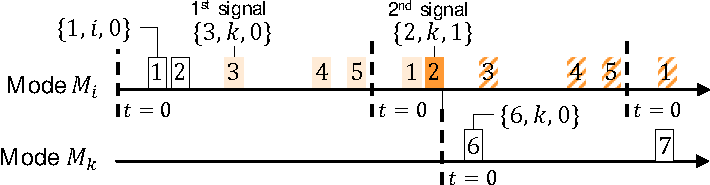
\includegraphics[scale=1]{mode_change}%
	\caption{%
	Example of mode change from mode \mode{i} to \mode{k}.
	\capt{%
	The dashed lines show the start of the mode hyperperiods.
	Each numbered box represents a communication round with its \id.
	The content of some of the host beacons is shown next to the corresponding rounds.
	In $r_3$, the host sends the first signal to change to mode \mode{k}. During this transition phase, the rounds are lightly colored.
	In the dark colored round, the host sets $\TB = 1$. This is the second signal -- directly after this round, mode \mode{k} starts executing.
	Dashed rounds are not executed.
	}
}
\label{fig:mode_change}
\end{figure}

\begin{example}
	Let us consider again the feedback control application from~\cite{mager2019Demo}.
	In this system, we implement a simple mode change protocol: all applications keep running until they are interrupted by a mode change.
%
	When a mode change is announced, a counter (initialized to 10) is appended to the beacon, and decremented with every round.
	The mode change is triggered (\ie \TB is set to~$1$) when the countdown reaches zero.
%
	With this approach, it is sufficient for any node to receive only one out of ten beacons to change mode at the correct time.
	Since the probability of reception of a packet is expected to be above 99\%~\cite{ferrari2011Glossy},
	receiving at least one out of ten beacons will happen with very high probability .
	Thus, this mode change protocol guarantees with very high probability that all the nodes in the system are always executing in the same mode, even in the occurrence of sporadic packet losses; this guarantees conflict-free communication across mode changes.
\end{example}

% !TEX root = ../00_thesis.tex

% ------------------------------------------------------------------------------
\section{Implementing \TTW}
\label{sec:ttw_implementation}
% ------------------------------------------------------------------------------

\TTW is a wireless \CPS design composed of two main building block:\linebreak
% (i)~
% \inlineitem
(i)~the system's communication backbone, which we call \TTnet ~(\cref{sec:ttw_overview}), and
% \linebreak
% (ii)~
% \inlineitem
(ii)~the \TTW scheduler, which synthesizes the timing of execution of all tasks, messages, and communication rounds~(\cref{sec:single_mode,sec:multi_mode}).
In this section, we describe how we implement \TTnet and the \TTW scheduler to obtain a fully functional \TTW system.
The performance of the implementation is discussed in \cref{sec:ttw_evaluation_sched,sec:ttw_evaluation_implem}.

% ------------------------------------------------------------------------------
\subsection{Implementation of \TTnet}
\label{subsec:implem_ttnet}

We implement \TTnet on embedded platforms built using the Dual-Processor Platform (\DPP) concept.
The \DPP links two arbitrary processors with a processor interconnect called \bolt~\cite{sutton2015Bolt}, which provides predictable asynchronous message passing between the two processors using message queues with first-in-first-out (FIFO) semantics, one for each direction.%
%
\footnote{Refer to the Introduction chapter for more details about the \DPP concept.}
%
The \DPP architecture is compatible with \TTW's system model, which assumes that a node is capable of performing one task execution and one message transmission simultaneously~(\cref{sec:model}):
We dedicate one processor (a TI MSP432~\cite{msp432}) to the execution of tasks and another one (a TI CC430 SoC~\cite{CC430F6137}) to wireless communication.
The \DPP platform we used is illustrated in~\cref{fig:dpp2-cc430}.

To implement the \TTnet network stack, we leverage the \baloo design framework~(introduced in \cref{ch:baloo}).
In particular, we use the ``static configuration'' mode of \baloo~(\cref{sec:adv_features}):
\TTW produces scheduling tables offline, which can be loaded in the nodes' memory to limit the runtime communication overhead~(\feature{Efficiency}).
The \TTnet beacons~(\cref{sec:ttw_overview}) are sent as \baloo control packets, using the customizable ``user-bytes'' field.%
%
\footnote{\href{https://github.com/ETHZ-TEC/Baloo/wiki/Baloo-control-packet}{github.com/ETHZ-TEC/Baloo/wiki/Baloo-control-packet}}


\begin{table}
  \centering
  \caption{Worst-case execution time of \bolt \opread and \opwrite functions}
  \label{table:boltAPIwcet}
  {\smaller \input{\TablePath/boltWCET.csv}}
\end{table}


To synthesize the schedules, one must know how long a communication round lasts.
For this purpose, the predictability of the \baloo framework is very beneficial: based on the implementation parameters, one can derive a precise estimate of the maximum possible length of a round.%
%
\footnote{The \TTnet model and its evaluation are presented in \cref{sec:ttw_evaluation_implem}.\label{footnote:ttnet}}
%
This model must account for the time to read and write messages over \bolt, the \DPP processor interconnect.
The \bolt API functions have formally verified semantics and bounded execution times~\cite{sutton2015Bolt}.
In our implementation, the two processors read and write over \bolt using the maximally supported SPI frequency of 4\MHz, leading to the worst-case execution times shown in \cref{table:boltAPIwcet}.
On the application side, we include the time to read and write messages within the WCET of tasks; in other words, we consider that a task ``starts'' when the processor initiates the \bolt \opread function, and terminates once the \bolt \opwrite function is completed.%
%
\footnote{Assuming that the task has some input and output messages.}
%
On the communication side, incoming messages are read from \bolt before the rounds. This is performed during the so-called ``pre-process'', which is scheduled before each \baloo round.%
%
\footnote{\href{https://github.com/ETHZ-TEC/Baloo/wiki/Baloo-pre-post-processes}{github.com/ETHZ-TEC/Baloo/wiki/Baloo-pre-post-processes}}
%
The messages received from the wireless network are written over \bolt directly after the communication slot, in \baloo's \texttt{on\_slot\_post()} callback function~(\cref{sec:baloo_implementation}).
Our implementation of \TTnet is available in the \baloo repository~\cite{repoBaloo}.



% ------------------------------------------------------------------------------
\subsection{Implementation of the \TTW Scheduler}
\label{subsec:implem_sched}

We implement the \TTW scheduler using Matlab~\cite{Matlab} and we use the Gurobi solver~\cite{Gurobi} for synthesizing the schedules.
All scripts are publicly available,%
%
\footnote{Although Matlab and Gurobi are commercial software, free academic and/or student licenses are currently available from the software vendors.}
%
together with details of the MILP formulation~(\cref{appendix:ttw_artifacts}).
In this section, we describe how to run the \TTW scheduler.

% \begin{itemize}
%
%   \item
  There are four high-level communication parameters that the user must specify in the \texttt{multimode\_main.m} file:
  \begin{itemize}[nosep]
    \item \customBox{$L$} The message payload size (in\bytes)
    \item \customBox{\nslotsmax} The maximal number of slots per round
    \item \customBox{$N$} The number of message transmissions in a Glossy flood~\cite{ferrari2011Glossy}
    \item \customBox{$H$} The estimated network diameter (in number of hops)
  \end{itemize}
  %
  % \item
  The \texttt{loadRoundModel.m} file contains the parameters of the \TTnet implementation~(\cref{subsec:implem_ttnet}). Combined with the high-level parameters described above, this allows the scheduler to compute the length of communication rounds.$^{\text{\ref{footnote:ttnet}}}$
  %
  % \item
  Finally, the user must specify the system's operation modes, applications, tasks, and messages, which is done by filling cell arrays in the \texttt{system\_configuration.m} and \texttt{mode\_configuration.m} files.
%
% \end{itemize}

\pagebreak

The scheduler supports user-defined constraints on the task and message offsets. These constraints must have the following form
\begin{equation}
  \sum_k \; \alpha_k*\mathit{id}_k.o \quad\mathit{`sign'}\quad \beta
\end{equation}
where $\mathit{id}$ is the unique identifier of a task or a message, $\alpha$ is a constant multiplier, $\mathit{sign}$ can be specified as `$=$' or `$<$', and $\beta$ is the right-hand side term of the constraint. The constraint may contain an arbitrary number of left-hand terms, denoted here by $k$.
These constraints are specified as tuples of the form
$  \{\,\{\mathit{id}_k,\, \alpha_k \}_k\,,\; \mathit{sign}\,,\; \beta \,\}$, as shown in~\cref{fig:user_constraints}; in that example, the user-defined constraints force some tasks to have the same offset; in other words, these tasks will execute simultaneously.
The user-defined constraints are automatically added to the MILP formulation; if the problem is feasible, the schedule is guaranteed to satisfy them.
Once all inputs have been specified, the schedules for all operation modes are synthesized and displayed by running the \texttt{multimode\_main.m} script.

\begin{figure}
{\smaller
\begin{lstlisting}%[caption = {Example of specification of user-defined constraint}]

CustomConstaints = { ...
    { {{'T_loc_stab1', 1},{'T_loc_stab2', -1}}, '=', 0}, ...
    { {{'T_loc_stab1', 1},{'T_loc_stab3', -1}}, '=', 0}, ...
    { {{'T_loc_stab1', 1},{'T_loc_stab4', -1}}, '=', 0}, ...
    { {{'T_loc_stab1', 1},{'T_loc_stab5', -1}}, '=', 0}, ...
    };
\end{lstlisting}}
\caption{Example of specification of user-defined constraints.
\capt{The generic formulation let the user define any linear constraint between the offsets of tasks and messages in the system. In this example, the constraints force all tasks \textup{\texttt{T\_loc\_stabX}} to have the same offset; in other words, these tasks will execute simultaneously.}}
\label{fig:user_constraints}
\end{figure}

% !TEX root = ../00_thesis.tex

% ------------------------------------------------------------------------------
\section{Performance of the \TTW Scheduler}
\label{sec:ttw_evaluation_sched}
% ------------------------------------------------------------------------------

The following two sections present the performance evaluation of our \TTW implementation, presented in~\cref{sec:ttw_implementation}.
We first evaluate the performance of the scheduler. In particular, we illustrate the benefits of the minimal inheritance strategy presented in \cref{sec:multi_mode} and we show that the complexity of the schedule synthesis is tractable.

% ------------------------------------------------------------------------------
\subsection{Benefits of Minimal Inheritance}

\begin{figure}
  \centering
  \href{\ttwfig{Figure-11}}{%
  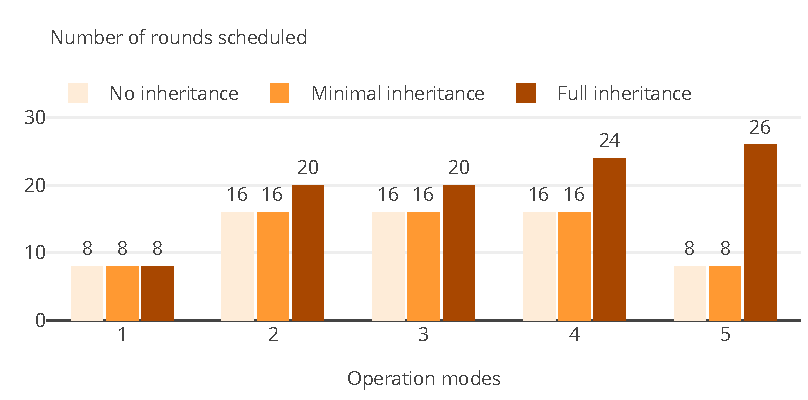
\includegraphics[scale=1]{inheritance_eval}}
  \caption{Number of rounds in the different modes' schedule, depending on the inheritance approach considered.
  \capt{We consider the number of rounds scheduled over 80\s, which is the least common multiple of the modes' hyperperiod.}}
  \label{fig:inheritance_eval}
\end{figure}

Every round introduces some overhead (mainly from  sending the beacon), which consumes energy.
To reduce the energy consumption, \TTW aims to minimize the number of rounds \objective{1}.
The schedule synthesis for a single mode is optimal in this respect; that is, the procedure guarantees that the schedule minimizes the number of communication rounds~(\cref{sec:single_mode}).

The second objective of the scheduler is to allow persistent applications to keep the same schedule in different operation modes \objective{2}.
This creates additional constraints that break the optimality guarantee: in other words, the schedule of mode \modej, when constrained to be compatible with mode \modei, may contain more rounds that required to schedule the mode \modej alone.
A naive solution to meet \objective{2} is to completely ``reserve the space'' of previously scheduled modes. This is equivalent to consider that all applications executing in mode \modei are also executing in \modej, even if it is not actually the case. We call this the \emph{full inheritance} approach.
This approach does guarantee compatibility but it is very pessimistic: it leads to an excessive increase of the number of rounds and find problems to be non-schedulable when they may in fact be feasible.


\begin{figure}
  \centering
  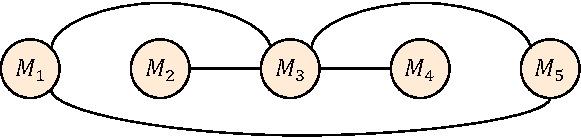
\includegraphics[scale=1]{modeGraph_eval}
  \caption{The mode graph \modeGraph' used in the inheritance evaluation scenario.
  Mode \modei has priority $i$. The applications executing in each mode are listed in~\cref{append:inheritance_eval}.}
  \label{fig:modeGraph_eval}
\end{figure}


In \cref{sec:multi_mode}, we derived the minimal set of constraints that are necessary to guarantee the compatibility between modes \objective{2}, which we refer to as \emph{minimal inheritance}.
We now illustrate with a simple example that the minimal inheritance does not overly increase the number of communication round required and performs much better than the full inheritance.
%
We consider the following configuration (fully detailed in \cref{append:inheritance_eval}): The system is composed of 13 nodes, running 15 different applications including 45 tasks and 30 messages.
The periods and deadlines vary between 10 and 80\s. The applications are executing in 5 different modes connected by the mode graph shown in~\cref{fig:modeGraph_eval}.
Finally, all applications are considered persistent.
We synthesize the schedule for the 5 modes while considering
(i)~no inheritance,%
%
\footnote{Considering no inheritance is equivalent to set all applications as non-persistent. In other words, there are no constraints between the different modes and the individual mode schedules are guaranteed to be optimal in terms of number of rounds~(\cref{sec:single_mode}).}
%
(ii)~our minimal inheritance approach, and (iii)~the naive full inheritance approach.
The results are shown in \cref{fig:inheritance_eval}.

One important observation is that the number of rounds steadily increases with the full inheritance approach, which is expected: the full inheritance assumes that all previously scheduled applications are still executing. Thus, the number of applications to schedule only increases, and so does the number of round required. Ultimately, this not only wastes energy, it also limits scalability with the number of operation modes.
In comparison, our minimal inheritance approach performs much better: Since only the required constraints are included, the minimal inheritance does not suffer from the scalability issue mentioned above. In this example, the minimal inheritance performs optimally (\ie it does not schedule more rounds that the minimum, captured by the ``no inheritance'' case); but note that this is {\bf not true in general}, it simply happens to be the case in this example.

\fakepar{Conclusion}
The minimal inheritance approach derived in \cref{sec:multi_mode} efficiently addresses the challenge of synthesizing compatible schedules~\objective{2} while minimizing the energy impact in terms of number of rounds scheduled~\objective{1}.
This approach does increase the complexity of the synthesis formulation; however, it is implemented in our \TTW scheduler, it induces no overhead for the user, and it does not affect the synthesis solving time, as discussed below.

% ------------------------------------------------------------------------------
\subsection{Offline Solving Time}

We computational complexity of the schedule synthesis is made tractable by \TTW's sequential approach: modes are scheduled individually, in order of priority~(\cref{sec:multi_mode}) and for each mode, the number of rounds to schedule is kept fixed then incremented until a solution is found~(\cref{sec:single_mode}).

For the evaluation scenario described above, the solving time for one mode grows up to ten minutes~(\cref{table:solvingTimes}) and is generally correlated with the complexity of the mode to schedule: mode \mode{3} and \mode{4} contains the most applications~(\cref{append:inheritance_eval}), leading to more constraints in the formulation.
Furthermore, we note that the minimal inheritance strategy does not increase the overall solving time compared to ``no inheritance''. The intuition is that, by reserving some applications' schedule, we fix the value of some of the problem variables, thereby reducing the complexity of the problem.
However, as shown by the full inheritance approach, if too many variables are fixed, the resulting problem might become harder to solve: more communication rounds become required, which increases the number of variables and thus the complexity.

\fakepar{Conclusion}
The evaluation scenario is simple but representative of a middle-sized \CPS. Our evaluation shows that the computational complexity may grow to the scale of minutes for challenging modes, which remains perfectly tractable for a task that needs to be performed only once and before deployment.

\begin{table}
  \centering
  \caption{Approximate solving time for the different modes of the inheritance evaluation~(\cref{sec:ttw_evaluation_sched}).
  \capt{Time expressed in seconds; all computation performed on a commodity laptop.}}
  \label{table:solvingTimes}
  {\smaller \input{\TablePath/solvingTimes.csv}}
\end{table}






% -----------------------------------------------------------------------------
\section{Performance of \TTnet}
\label{sec:ttw_evaluation_implem}
% ------------------------------------------------------------------------------

After the evaluation of the \TTW scheduler~(\cref{sec:ttw_evaluation_sched}), we now consider the performance of our \TTnet implementation, described in \cref{subsec:implem_ttnet}.

% ------------------------------------------------------------------------------
\subsection{Memory Utilization}

First, we consider the memory utilization induced by storing the scheduling tables in the nodes' memory.
For a given operation mode, the entire schedule contains the task offsets, the message offsets and deadlines, the round starting times, and the allocations of messages to rounds~(\cref{table:ttw_inputs_outputs}).
In addition, nodes must know the task periods and the mode hyperperiod to compute the absolute start time of the tasks and rounds.

Since we dedicate the execution of tasks and the wireless communication to different processors~(\cref{sec:ttw_implementation}), the memory cost for storing the schedule can be splitted.
On the application side, we must store the task offsets and periods, which are required to know when to execute the tasks; \ie 2 variables per task.
On the communication side, we must store the mode hyperperiod and the rounds information, \ie the offset and allocation of the rounds scheduled within the mode's hyperperiod; \ie $(\nslotsmax+1)$ variables per round.
The message deadlines are not required at runtime and do not need being stored.
As a result, we can generally estimate that the scheduling tables represent tens to hundreds of variables per mode for each processor.

\fakepar{Conclusion}
Our application and communication processors feature 64\kB~\cite{msp432} and 4\kB\cite{CC430F6137} of RAM, respectively. Thus, considering an average size of two\bytes per variable, storing the scheduling tables represent a significant overhead and limits the scalability of the system, in particular on the communication processor.
This limitation would be significantly relaxed with newer platforms, which commonly feature 256\kB of RAM~\cite{nRF52840}.

% ------------------------------------------------------------------------------
\subsection{\TTnet Model}
\label{subsec:model}
As discussed in \cref{sec:ttw_implementation}, we implement \TTnet using \baloo, which allows to derive a precise model of
(i)~the execution time of a communication round and
(ii)~the time spent with the radio turned on, which correlates with the energy consumed for communication.
Estimating the communication time is necessary to synthesize the schedules since the scheduler must know how long the rounds last.
This model should be as tight as possible not to ``waste'' time and thus minimize the end-to-end deadlines schedulable by \TTW, but it must be a safe upper-bound in order to prevent deadline misses.
This section presents our \TTnet model and derives the theoretically achievable performance in terms of minimal message latency and the energy savings expected from using rounds.

Let $\app.\delta$ denote the latency of an application \app. This latency represents the delay for a complete execution of \app; that is, the completion of all tasks in \app.\predG. Let $\app.c$ be a \emph{chain} in \app.\predG.
A chain is defined as a path of \app.\predG starting with a task without predecessor and ending with a task without successor.%
%
\footnote{For example, $(\tau_2, m_2, \tau_4)$ is a chain of \predG in \cref{fig:precedence_graph}.}
%
The minimum achievable latency for a single message in \TTW is the length of a round composed of only one slot, denoted $\Tround(L,1)$ where $L$ is the payload size. Thus $\app.\delta$ is lower-bounded by
\begin{align}
\label{eq:min_deadline}
\app.\delta \;
	& \geq \; \max_{\app.c \,\in\, \app.\predG}
		\left(
			\; \sum_{\tau \, \in \, \app.c} \tau.e \,+\, \sum_{m \, \in \, \app.c} \Tround(L,1) \;
		\right)
\end{align}

\begin{remark}
  By comparison, the best possible guarantee for the latency of a single message provided by  \DRP~(\cref{ch:drp}) is of the order of $2*\Tround(L,\nslotsmax)$.
  Since $\Tround(L,\nslotsmax) \approx \nslotsmax*\Tround(L,1)$, \TTW reduces the minimal guarantee on message latency by a factor of approximately $2*\nslotsmax$.
  For a relatively small number of slots per round, such as $\nslotsmax=5$, this represents an order of magnitude improvement.
  This difference stems from the loose coupling between the task and message schedules in \DRP, whereas \TTW statically schedules all tasks and messages.
\end{remark}


\afterpage{
\begin{figure}
\centering
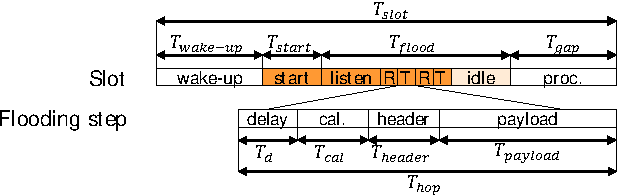
\includegraphics[scale=1]{Tslot}
\caption{%
Break-down of a communication round.
\capt{%
At the slot level, the colored boxes identify phases where the radio is on.
In the ``idle'' phase, the radio is turned off in practice, but this idle time depends on each node's distance to the initiator.
To estimate the energy saving of rounds (\cref{fig:energy_ratio}), we assume that the radio stays on for the whole time of \Tglossy, as specified in~\cref{eq:Ton}.
}
}
\label{fig:Tslot}
\end{figure}}

A round \Tround is composed of up to $(\nslotsmax+1)$ slots in which Glossy floods~\cite{ferrari2011Glossy} are executed.
An entire slot completes in time $\Tslot$, decomposed into
\begin{equation}
  \Tslot = \Twakeup + \Tstart + \Tglossy + \Tgap
\end{equation}
The composition of a slot in our implementation is detailed in~\cref{fig:Tslot}.
First, all nodes wake up (\Twakeup) and switch on their radio (\Tstart).
Then the message flood starts. We denote by \Thop the time required for one protocol step, \ie a one-hop transmission. The total length of the flood is
%
\begin{align}
\Tglossy = (H+2N-1)*\Thop
\end{align}
with $H$ the network diameter and $N$ the number of times each node transmits each packet.%
%
\footnote{Glossy achieves more than 99.9\% packet reception rate using $N =2$~\cite{ferrari2011Glossy}.}
%
\Thop is itself divided into
%
\begin{align}
\Thop = \Td + \Tcal + \Theader + \Tpayload
\end{align}
where \Td is a radio delay, and \Tcal, \Theader and \Tpayload are the transmission times of the clock calibration message, the Glossy header and the message payload, respectively.
With a bit rate of \Rbit, the transmission of $L$\bytes takes
%
\begin{align}
T(L) = 8L/\Rbit
\end{align}
Once the flood is completed, some gap time \Tgap is necessary to process the received packet.
This time is used (among other things) to execute \baloo's \texttt{on\_slot\_post()} callback, where the received messages are written into \bolt.
We divide \Tslot into \Ton and \Toff, which denote the time spent with radio on and off, respectively.
%
\begin{align}
\Toff &\,=\,
	\Twakeup + \Tgap \\
\nonumber
\Ton(L) &\,=\,
	\Tstart + \\
\label{eq:Ton}
  & \qquad (H+2N-1) * \left( \Td + 8(\Lcal + \Lheader + L)/\Rbit \right) \\
\Tslot(L) &\,=\,
  \Toff + \Ton(L) \\
\Tround(L)
	&\,=\,
	\Tslot(\Lbeacon) + B*\Tslot(L) + \Tpreprocess
\end{align}

Sending beacons is necessary to let the nodes know about the current state of the system; \ie which mode is executing and ``how far'' is the system in the scheduling table. Without that information, it is impossible for a failing node to recover and resume its normal operation.
Moreover, beacons prevent message collisions by guaranteeing that the nodes always know the system's state when a round starts.
In a design \emph{without} round, each message transmission should be preceded by its own beacon to provide the same guarantees. Thus, the transmission time for \nslots messages of size $L$, denoted $\Tworound(L)$, would take
%
\begin{align}
\Tworound(L) =  B*( \, \Tslot(\Lbeacon) + \Tslot(L) \, )
\end{align}
%
We can then derive the relative energy savings $E$ granted by using a round-based design, which we compute as $E= (\Tworoundon - \Troundon)/\Tworoundon$.


\afterpage{
\begin{figure}
  \begin{subfigure}{\linewidth}
    \centering
    \href{\ttwfig{Figure-14}}{%
    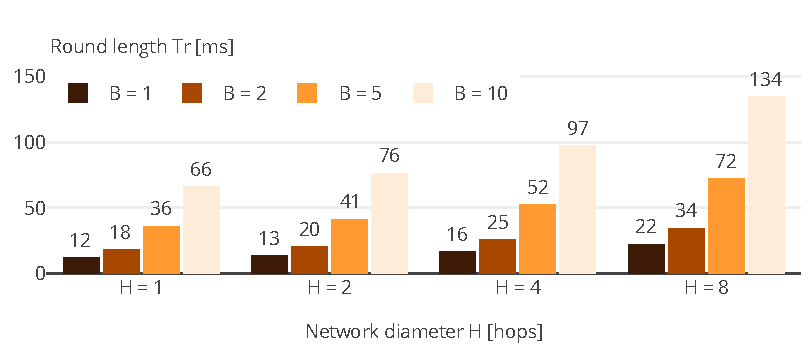
\includegraphics[scale=1]{T=f(H,B)}}
  \end{subfigure}
  \begin{subfigure}{\linewidth}
    \centering
    \href{\ttwfig{Figure-14}}{%
    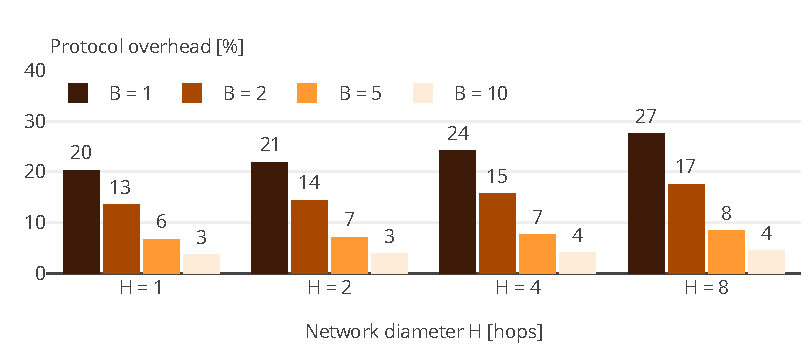
\includegraphics[scale=1]{Overhead=f(H,B)}}
  \end{subfigure}
  \caption{Example values of round length (top) and protocol overhead (bottom) computed using the \TTnet model~(\cref{subsec:model}).
  The protocol overhead is computed as the percentage of time spent to send the beacons relative to the overall communication time for a round containing \nslots slots.
  Payload is set to 16\bytes and we use $N = $2 transmissions in the Glossy floods~\cite{ferrari2011Glossy}.}
  \label{fig:TTWmodel}
\end{figure}
}


The complete \TTnet model is available in Appendix~(\cref{appendix:ttw_artifacts}). We use this model to compute the round length \Tround and the energy savings $E$ for different values of number of slots per rounds (\nslots), message payload size ($L$), network diameter $H$, and number of transmissions in Glossy floods ($N$).
Selected results are shown in \cref{fig:TTWmodel,fig:energy_ratio}.
\linebreak
For example, with $N$ set to 2, it takes less than 100\ms to complete a 10-slot round sending 16-bytes messages over a 4-hop network~(\cref{fig:TTWmodel}, top).



% ------------------------------------------------------------------------------
\subsection{Model Validation}

We now evaluate the runtime execution of our implementation and aim to validate our \TTnet model.
In particular, it is important that the round length model gives safe upper-bounds since the \TTW scheduler relies on the model to schedule messages and tasks: if a round overruns, this may delay the execution of subsequent tasks and cause deadline misses.
We test our \TTnet implementation for different number of slots per round \nslots and payload size $L$, we measure the round length and radio-on time experienced by the different nodes in the network, and we compare the results with the \TTnet model.

\fakepar{Evaluation scenario}
We program the network to execute, one round with \nslots slots, followed by \nslots rounds with one slot.
For each of these rounds, we collect the round length and the radio-on time. Both values are measured in software (\ie the measurement is implemented in the firmware) and use a 32\kHz timer, leading to a measurement accuracy of about 30\us.

\begin{table}
  \centering
  \caption{\triscale parameters for the experimental validation of \TTnet's model}
  \label{table:ttw_triscale_param}
  {\smaller \input{\TablePath/triscale_param.csv}}
\end{table}


\fakepar{Experiment design}
We design the evaluation using the \triscale framework (introduced in \cref{ch:triscale}). The evaluation parameters are listed in \cref{table:ttw_triscale_param}.
Our evaluation scenario is terminating (there is a finite task to accomplish); thus there is no need to test for convergence.
The round length evaluation aims to validate that the \TTnet model is a safe upper-bound; thus, we use the maximum measured round length across all nodes as metric for a run.
For the same reason, we choose a large KPI (95th percentile) and a high confidence level (95\%), which leads to a minimal number of 59 runs per series.
To investigate the reproducibility of the results, we choose the median and a 75\% level of confidence for the variability scores, leading to a minimal number or 3 series.
To evaluate the average savings provided by using communication rounds, we use the median values across nodes as metric.
We perform the evaluation on FlockLab~\cite{FlockLab}, an indoor testbed located in an office building. It has been shown that the experimental conditions on FlockLab exhibits weekly seasonal components~(\cref{subsec:network_profiling}); therefore, to avoid biasing our evaluation, we perform our series of runs using a span of one week, during which we schedule randomly 60 runs per set of parameters. We test our \TTnet implementation using 5, 10, and 30 slots per round, and payloads of 8, 16, and 64\bytes.
The three series of tests were performed between May and October 2019.
The KPI values from our evaluation are listed in~\cref{table:KPIs}.

\afterpage{
\begin{figure}
  \centering
  \href{\ttwfig{Figure-15}}{%
  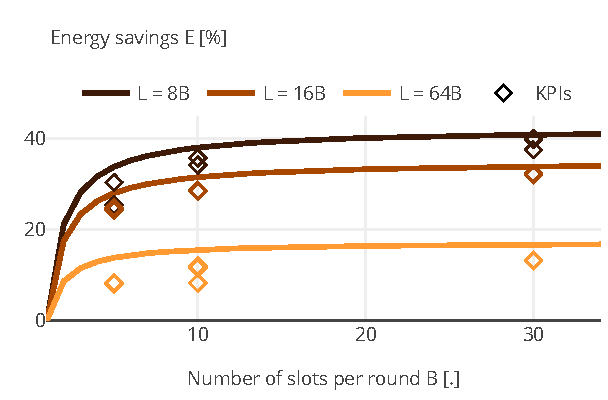
\includegraphics[scale=1]{energy_savings}}
  \caption{Relative radio-on time savings by using rounds compared to single messages.
  \capt{The energy savings induced by a round-based design grow with the number of number of slots per round (X-axis). Conversely, these savings become less significant as the payload size increases (lighter colors).
  The diamonds show our evaluation KPIs and thus estimate, with a probability of 95\%, the average energy savings expected in 95\% of the test runs. $H = 4$, $N = 2$.}}
  \label{fig:energy_ratio}
\end{figure}}

\begin{remark}
  Observe that certain values in~\cref{table:KPIs} are reported with a {\ssymbol{1}} or {\ssymbol{2}} symbol.
  The {\ssymbol{1}} marks series where \triscale independence test fails; this indicates that the metric data do not appear to be \iid and therefore the KPI value loose its predictive power (\ie it does not allow to infer what is the expected performance).
  However, in our evaluation, the autocorrelation plots show no significant differences between the series that passes the test and those that do not~(data available in~\cref{appendix:ttw_artifacts}).
  Moreover, the round length KPI values are almost the same in all series.
  Together, these two facts increase our confidence in the results and suggests that the reported KPIs are robust estimates of the expected performance.\\
  The {\ssymbol{2}} marks series where we could not collect enough data in order to compute the KPIs. This appended in Series 3 due to construction work taking place in the FlockLab building, where many test runs were lost due to sporadic power outages.
  In both cases, the table shows the maximum round length or minimum energy savings metric values obtained across all the runs in the series.
\end{remark}

\fakepar{Results -- Round length}
The results for the round length are extremely stables~(\cref{table:KPIs}):
the differences of KPI values between series are at most one time tick ($\approx$ 30\us), which is our measurement accuracy.
Concretely, this means that, in all series, the largest round length measured by any node is essentially the same.

Furthermore, the KPI values are (i)~very close to and (ii)~consistently lower than the model. By definitions of the KPI, we can estimate with 95\% probability that (at least) 95\% of runs will yield a maximal round length smaller than the KPI value, and thus smaller than the model value.
\cref{fig:exampleSeries} (top) shows the distribution of the round length measurements from all the nodes collected during one series of 60 runs. We observe that the distribution is narrow (less than 300\us of spread), which is expected. Indeed, the \TTnet rounds are fully time-triggered; thus, the measurement differences between nodes mainly come from the difference in execution time of \baloo's end-of-round operations, which is expected to be small.

In our entire evaluation, there was one case where a node reported a value (77.85\ms) larger than the model (77.52\ms). This concerned only one node: in this run%
\footnote{FlockLab test number 66992; data available in~\cref{appendix:ttw_artifacts}.}
the second highest value reported (77.12\ms) was smaller than the model value.
It is hard to know a posteriori what may have cause this.
However, we argue that this one overshoot is more likely imputable to some sporadic hardware delay than due to a miscalibration of the model.

\afterpage{
\begin{figure}
  \centering
  \begin{subfigure}{\linewidth}
    \centering
    \href{\ttwfig{Figure-16}}{%
    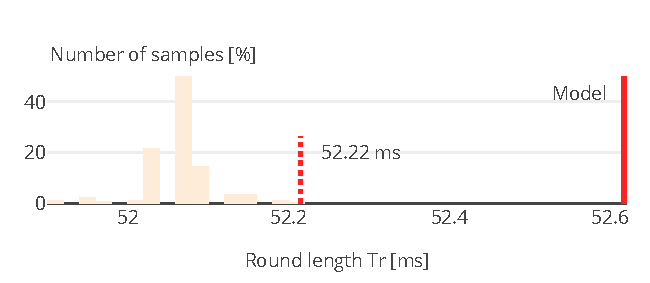
\includegraphics[scale=1]{serie2_T_round_H4_N2_L16_B5}}
  \end{subfigure}
  \begin{subfigure}{\linewidth}
      \centering
      \href{\ttwfig{Figure-16}}{%
      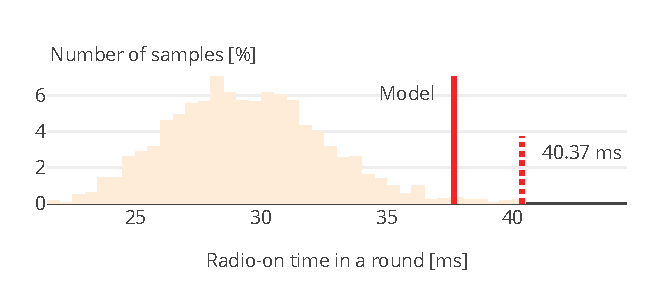
\includegraphics[scale=1]{serie2_T_on_round_H4_N2_L16_B5}}
  \end{subfigure}
  \caption{Distributions of round length (top) and radio-on time (bottom) measurements from all the nodes, collected in one series of 60 runs (Serie 2, $L=16$, $\nslots=5$).
  \capt{
    While the distribution of round length is very narrow, the radio-on time exhibits a much larger spread. We can see that the \TTnet model provides a generally overestimate the radio-on time, which is expected since it assumes that nodes keep their radio on for the entirety of \Tflood~\textup{(}\cref{eq:Ton}\textup{)}, which is not the case in practice: nodes turn the radio off when they have transmitted a packet $N$ times.
  }}
  \label{fig:exampleSeries}
\end{figure}}

\fakepar{Results -- Energy savings}
The energy savings results show more fluctuations than the round length, which is not surprising: (i)~the energy model is less precise and (ii)~the dynamic interference conditions affect the radio-on time, as nodes may need to keep their radio on for a longer share of \Tglossy.
\cref{fig:energy_ratio} shows the model and our energy savings KPIs together.
\cref{fig:exampleSeries} (bottom) shows the distribution of radio-on time measurements from all the nodes, collected in one series of 60 runs: nodes experience significant differences in radio-on time during a round. This is expected since nodes terminate a flood as soon as they have transmitter a packet $N$ times, which happens earlier for nodes that are closer to the initiator,

Overall, the energy savings come from the ``distribution'' of the overhead from sending beacons between the slots. Thus, the more slots (increasing \nslots) and the smaller the slots (decreasing $L$), the more radio-on time is spared by using rounds.
For a payload of 16\bytes, we obtain an average energy savings of about 30\% with only 10 slots per round.

\afterpage{
\begin{landscape}
\begin{table}
  \centering
  \caption{
  KPIs from the performance evaluation described in~\cref{sec:ttw_evaluation_implem} and corresponding model values for the \TTnet round length \Tround and energy savings $E$; other settings: $H=4$ and $N=2$.
  \capt{
    The value marked in bold corresponds to the one case where the round length KPI is larger than the model value.
    {\ssymbol{1}} marks series where \triscale independence test failed.
    {\ssymbol{2}} marks series without enough samples for computing the KPIs.
    In these two cases, reported values are the maximum round length or minimum energy savings metric values for all the runs in the series.
  }}
  \label{table:KPIs}
  {\smaller \input{\TablePath/KPIs.csv}}
\end{table}
\end{landscape}
}

\fakepar{Conclusion}
We validated the tightness and safeness of \TTnet round length model, which was found to be an upper-bound of the effective round length for all but one in about 14k measurements collected.
Furthermore, we showcased that, even with small beacons (2\bytes in our implementation), a round-based design yields significant reduction of radio-on time, and therefore helps minimizing the overall energy consumption~(\feature{Efficiency}).

% !TEX root = ../00_thesis.tex
\section{Discussion, Limitations, and Future Work}

\fakepar{Debugging the scheduler is hard}
When a system configuration is found unfeasible by the \TTW scheduler, it is not easy to identify which of the constraints are responsible. Our scheduler implementation would benefit from better built-in support to turn the IIS (irreducible constraint set, returned by the Gurobi solver) into a legible output for the user.

\squarepar{%}
  \fakepar{The multi-mode scheduling strategy is not complete}
  Even with our minimal inheritance approach~(\cref{sec:multi_mode}), the \TTW scheduler may find a problem unfeasible even though a solution exists.
  This is due to the sequential synthesis of schedules, which is a generally under-defined problem: the choices made when synthesizing a mode's schedule may make lower-priority modes unfeasible.
  Completeness (the guarantee to find a solution if one exists) can be obtained by synthesizing all schedules within a single MILP formulation; however, the complexity scales exponentially with the number of variables~\cite{jeffay1991nonpreemptive}, which limits the practicality of this ``one-shot'' approach.
  Another alternative would be to leverage the IIS information to iterate on previously scheduled modes.
  This is not trivial and, in particular, the scheduler must be careful not to search forever
  shall the system configuration would be truly unfeasible.%
}

In practice though, the lack of completeness is not a critical problem. If one mode \modeany is found unfeasible, a practical work-around is to add the conflicting applications (derived from the IIS) to the specification of \modeany.
This triggers the minimal inheritance mechanism and prevents conflicts in mode \mode, at a cost of an increase in utilization.

\fakepar{Integration of \TTnet with the \TTW scheduler}
We presented in \cref{sec:ttw_implementation} our implementation of \TTnet and the offline \TTW scheduler.
To obtain a full-fledged \TTW implementation, one needs to integrate these two pieces. Concretely, that means designing a pipeline that turns the outputs of the \TTW scheduler into individual nodes' scheduling tables, which can be then patched in the \TTnet firmware.
There is no technical limitation in realizing this; it could not be done in time before the completion of this dissertation, but we intend to make this happen in the near future.

\squarepar{%}
  \fakepar{Showcasing the full feature set of \TTW}
  A running implementation of the \TTW concept, including switching between operation modes, has been presented in the 2019 IPSN Demo Session~\cite{mager2019Demo}. This demo ran a more static and rigid software than the implementation presented in this chapter. Furthermore, all applications were considered non persistent; in other words, applications were re-starting from scratch with every mode change.\linebreak
  A demonstration of the full feature set of \TTW remains to be done.

  \fakepar{Porting to other platforms}
  Our implementation of \TTnet currently supports the TI CC430 SoC~\cite{CC430F6137}, which is not a commonly used platform and features only little memory.
  Porting \TTnet to newer platforms would be beneficial, and this is made simple by the use of the \baloo framework: whenever \baloo becomes available for a new platform, so does \TTnet.
  In particular, a port to the nRF52840 Dongle~\cite{nRF52840} is envisioned, which would provide a physical layer (up to) 8x faster (and therefore, support for shorter end-to-end deadlines) and larger memory, which would facilitate the storing of scheduling tables.%
}

\fakepar{Adaptability by reprogramming}
The main limitation of \TTW is that the schedules are static: the system executes pre-computed scheduling tables stored in the nodes' memory, with runtime adaptability limited to switching between different operating modes.
However in principle, \feature{Adaptability} could be improved by specifying a ``reprogramming'' mode in which new scheduling tables could be disseminated to the network to perform some sort of over-the-air reprogramming~\cite{hagedorn2008Rateless}.
Doing this reliably is challenging and would be an interesting extension of this work.

% !TEX root = ../00_thesis.tex

\section{Related Work}
\label{sec:ttw_relWork}

Various high reliability protocols have been proposed for low-power multi-hop wireless network, like TSCH~\cite{watteyne2017Teaching}, WirelessHART~\cite{wirelessHART} or LWB~\cite{ferrari2012LWB}.
Blink~\cite{zimmerling2017Blink} was proposed as a real-time scheduling extension for protocols based on synchronous transmissions.
Despite their respective benefits, all these protocols consider only network resources. They do not take into account the scheduling of distributed tasks on the computation resources, and therefore they hardly support end-to-end deadlines as commonly required for \cps applications~\cite{akerberg2011Future}.
In \cref{ch:drp}, we proposed \DRP a protocol that provides such end-to-end guarantees, but couples tasks and messages as loosely as possible, aiming for efficient support of sporadic or event-triggered applications.
This results in high worst-case latency and is thus not suitable for demanding \cps applications~\cite{akerberg2011Future}.
This observation points toward a fully time-triggered system where tasks and messages are co-scheduled.


In the wired domain, much work has been done on time-triggered architecture, like TTP~\cite{kopetz1993TTP}, the static-segment of FlexRay~\cite{flexray2013ISO}, or TTEthernet~\cite{kopetz2005TimeTriggered}.
Many recent works use SMT- of MILP-based methods to synthesize and/or analyze static (co-)schedules for those architectures~\cite{steiner2010evaluation,craciunas2016Combined,ashjaei2017Designing,tamas2012Synthesis,zhang2014Task}.
However, these approaches assume that a message can be scheduled at any time. While being a perfectly valid hypothesis for a wired system, this assumption is not compatible with the use of communication rounds in a wireless setting.
As shown in \cref{sec:ttw_evaluation_implem}, using rounds significantly reduces the energy consumed for communication, but it makes the schedule synthesis more complex~(\cref{sec:single_mode}).

% !TEX root = ../00_thesis.tex

\section{Summary}
\label{sec:ttw_conclusion}

%What we presented
In this chapter, we presented Time-Triggered Wireless (\TTW), a time-triggered design for wireless \CPS.
\TTW provides end-to-end real-time guarantees by statically co-scheduling all tasks and messages in the system, which is performed offline by resolving a MILP formulation.
This approach is inspired by similar work in the wired domain, in particular the real-time scheduling of FlexRay buses.
Compared to \DRP~(\cref{ch:drp}), \TTW's static schedules allow to meet shorter end-to-end deadlines \feature{Efficiency} at the cost of a lesser (\feature{Adaptability}); indeed, \TTW's runtime adaptability is limited to switching between pre-defined operation modes.

% Key concept/novel idea
\squarepar{%}
  The main challenge in the \TTW design is that, with wireless communication, it is highly beneficial in terms of energy to send messages in rounds. Thus, the assignment of messages to round (similar to a bin-packing problem) must be combined to the traditional co-scheduling approaches, which is non-trivial.

  % Take aways
  We solved this problem and implemented a multi-mode scheduler that allows critical applications to seamlessly switch between modes while minimizing the energy consumption spent for wireless communication.
  We further implemented a predictable network stack, called \TTnet. Together, these two pieces from \TTW, a publicly available~(\cref{appendix:ttw_artifacts}) real-time wireless \CPS design.%
}


% Chapter appendices
\begin{subappendices}
  \newpage
  % !TEX root = ../00_thesis.tex
\section{Appendix -- Artifacts and Links}
\label{appendix:ttw_artifacts}

\subsection{Related Publications}

\inlineRef%
{TTW: A Time-Triggered Wireless design for CPS}%
{Romain Jacob, Licong Zhang, Marco Zimmerling, \\Jan Beutel, Samarjit Chakraborty, Lothar Thiele}%
{DATE 2018. Dresden, Germany (March 2018)}

\customLink{\IconPaper}{Paper}{10.23919/DATE.2018.8342127}{https://doi.org/10.23919/DATE.2018.8342127}
\customLink{\IconPaper}{Extended paper}{arxiv.org/abs/1711.05581v2}{https://arxiv.org/abs/1711.05581v2}
\customLink{\IconPoster}{Poster}{10.3929/ethz-b-000375611}{https://doi.org/10.3929/ethz-b-000375611}

\inlineRef%
{The Time-Triggered Wireless Architecture}%
{Romain Jacob, Licong Zhang, Marco Zimmerling, \\Jan Beutel, Samarjit Chakraborty, Lothar Thiele}%
{ECRTS 2020. Modena, Italy (July 2020)}

\customLink{\IconPaper}{Paper}{10.4230/LIPIcs.ECRTS.2020.19}{https://doi.dx/10.4230/LIPIcs.ECRTS.2020.19}

\subsection{Complementary Materials}
Complementary materials for this chapters are available on GitHub, together with the dissertation source files. For all links below, replace
\linkroot  by ``{github.com/romain-jacob/doctoral-thesis/blob/master}''

\customLink{\IconTex}{\tex sources}{\linkroot/50\_TTW/}{\linkrootURL/50\_TTW/}

\customLink{\IconPlot}{Figures}{}{}
  \customLink{}{--- Static}{\linkroot/50\_TTW/Figures/}{\linkrootURL/50\_TTW/Figures/}
  \customLink{}{--- Dynamic}{\linkroot/notebooks/ttw\_plots.ipynb}{\thesisroot/ttw\_plots.ipynb}

\customLink{\IconData}{\TTW Artifacts}{}{}
  \customLink{}{--- GitHub}{romain-jacob/TTW-Artifacts}{https://github.com/romain-jacob/TTW-Artifacts}
  \customLink{}{--- Latest release}{10.5281/zenodo.3759221}{https://doi.org/10.5281/zenodo.3759221}

\customLink{\IconCode}{\TTnet source code (examples/baloo-ttnet)}{}{}
  \customLink{}{--- Latest release}{10.5281/zenodo.3510171}{https://doi.org/10.5281/zenodo.3510171}
  \customLink{}{--- ``This-version'' release}{10.5281/zenodo.3530632}{https://doi.org/10.5281/zenodo.3530632}

\pagebreak

\customLink{\IconCode}{\TTW Scheduler (sources and documentation)}{}{}
  \customLink{}{--- Latest release}{10.5281/zenodo.3530665}{https://doi.org/10.5281/zenodo.3530665}
  \customLink{}{--- ``This-version'' release}{10.5281/zenodo.3530666}{https://doi.org/10.5281/zenodo.3530666}

\customLink{\IconDataset}{\TTnet Model Validation data}{}{}
  \customLink{}{--- Latest release}{10.5281/zenodo.3530721}{https://doi.org/10.5281/zenodo.3530721}
  \customLink{}{--- ``This-version'' release}{10.5281/zenodo.3530722}{https://doi.org/10.5281/zenodo.3530722}

  % \newpage
  % % !TEX root = ../00_thesis.tex

\section{Appendix -- MILP Formulation}
\label{appendix:single_mode}

\TODO{read carefully (will need to be adapted to the new sched synthesis) and potential merge with the tech report version}

This appendix presents the complete description of the ILP formulation, used to synthesize the schedule \sched{\mode{}} of a given operation mode \mode{}, \ie
\begin{align*}
&\sched{\mode{}} \; = \;
	\left\lbrace
	\begin{tabular}{c@{\quad}|@{\quad}l}
	$\tau.o, \, m.o, \, m.d$
	&
	$\app \in \mode{}, \;
	(\tau,m) \in \app.\predG$
	\\
	$r_k.t, \, r_k.[B]$
	&
	$k \in [1, \, R_{\mode{}}]$
	\end{tabular}
	\right\rbrace
\end{align*}


The system model is described in \cref{sec:model}. All the variables and parameters involved in the ILP formulation used to solve the single-mode schedule synthesis problem are listed at the end in Table~\ref{tab:ILPvar} for reference.
This appendix details all the formulated constraints and how they are implemented in practice. The last subsection details the formulation of the objective function used to minimize the end-to-end application latency.

%%1. Pseudo-code that shows how we guarantee that the number of rounds is minimized
%The schedule of a mode \mode{} is computed for one hyperperiod, after which it repeat itself.
%To minimize the number of rounds used, we solve the problem sequentially, as described in Alg.~\ref{alg:outerlayer}.
%Each ILP formulation considers a fixed number of rounds $R_{\mode{}}$ to be scheduled, starting with $R_{\mode{}}=0$. The number of rounds is incremented until a feasible solution is found, or until the maximum number of rounds $R_{max}$ -- the number of rounds that ``fit'' into one hyperperiod -- is reached.
%Thus, Alg.~\ref{alg:outerlayer} guarantees by construction that if the problem is feasible, the synthesized schedule is optimal in terms of number of rounds used.
%The end-to-end latency is minimized by setting the sum of all application's latency as objective function.
%
%
%\begin{algorithm}
%\begin{algorithmic}
%\small
%\Require
%	mode \mode{},
%	applications $\app \in \mode{}$,
%	task mappings $\tau.map$ and WCETs $\tau.e$,
%	round duration $\Tround$
%	\; -- \;
%\textbf{Output:}
%	\sched{M}
%
%\State $LCM \gets$ \textit{hyperperiod}(\mode{})
%%\State $R_{min} = 1$
%\State $R_{max} = floor(LCM/\Tround)$
%
%\State $R_{\mode{}} = 0$
%
%\While{$R_{\mode{}} \leq R_{max}$}
%	\State formulate the ILP for mode \mode{} using $R_{\mode{}}$ rounds
%%	ILP = \textit{pbmFormulation}( \mode{} , $R$ )
%	\State [ \sched{M}, \textit{feasible} ] = \textit{solve}( ILP )
%	\If {\textit{feasible}}
%		\Return \sched{M}
%	\EndIf
%	\State $R_{\mode{}} \gets R_{\mode{}}+1$
%\EndWhile
%\State \Return 'Problem unfeasible'
%\end{algorithmic}
%\caption{Pseudo-code of the schedule synthesis}
%\label{alg:outerlayer}
%\end{algorithm}


The ILP formulation to be solved by Alg.~\ref{alg:outerlayer} (see \cref{sec:model}) contains the following constraints, which can be classified into four categories.

\fakepar{1. Application constraints}
		\begin{description}
			\item[(C1.1)] Precedence constraints between tasks and messages must be respected.
			\item[(C1.2)] End-to-end deadlines must be satisfied.
		\end{description}

\fakepar{2. Round constraints}
		\begin{description}
			\item[(C2.1)] The rounds must not be overlapping.
			\item[(C2.2)] The time interval between two rounds is upper-bounded.
		\end{description}

\fakepar{3. Validity of the tasks mapping}
		\begin{description}
			\item[(C3)] The same node cannot process more than one task simultaneously.
		\end{description}

\fakepar{4. Validity of the messages allocation}
		\begin{description}
			\item[(C4.1)] Every message must be served
			after its release time.
			\item[(C4.2)] Every message must be served
			before its deadline.
			\item[(C4.3)] A round cannot be allocated more messages than the number of slots available in one round.
			\item[(C4.4)] Within one hyperperiod, the same number of messages are released and served.
		\end{description}

The validity of the message allocation constraints, in particular constraints \textbf{(C4.1)} and \textbf{(C4.2)}, induce a non-linear coupling between the message and round variables. This peculiar aspect makes the scheduling problem non-trivial and prevents the use of conventional ILP-based schedule synthesis approaches reported thus far in the literature.
Our approach to solve this problem is detailed in \cref{sec:message_alloc}.


\subsection*{Application constraints}\label{sec;application}
\begin{description}
	\item[(C1.1)]Precedence constraints between tasks and messages must be respected.
\end{description}
For any application \app, let $\app.c$ be a \emph{chain} in \app.\predG. A chain is a path of \app.\predG starting and ending with a task without predecessor and successor, respectively. $\app.c(\,\first\,)$ and $\app.c(\,\last\,)$ denote the first and last task of the chain \app.c.  $\sigma_{i,j}$ is a binary variable accounting for the cases where successive task $\tau_i$ and message $m_j$ (resp. a message $m_i$ and task $\tau_j$) start during different application period ($\sigma_{i,j} = 1$) or not ($\sigma_{i,j} = 0$)
\begin{align}
\intertext{%
$	\forall\, \app, \;
	\forall\, \app.c \in \app.\predG, \;
	\forall\, \tau_j \in (\app.c \setminus \app.c(\,\last)),\;
	\forall\, m_i \in \tau_j.prec,
	$}
		m_i.o + m_i.d
		&\;\leq\; \app.p * \sigma_{i,j} + \tau_j.o\\
\intertext{%
$	\forall\, \app, \;
	\forall\, \app.c \in \app.\predG, \;
	\forall\, m_j \in \app.c,\;
	\forall\, \tau_i \in m_j.prec,
	$}
		\tau_i.o + \tau_i.e
		&\;\leq\; \app.p * \sigma_{i,j} + m_j.o
\end{align}

\begin{description}
	\item[(C1.2)] End-to-end deadlines must be satisfied.
\end{description}
\begin{align}
\intertext{%
$	\forall\, \app, \;
	\forall\, \app.c \in \app.\predG, \;
		\tau_{\first} = \app.c(\,\first\,), \;
		\tau_{\last} = \app.c(\,\last\,), \;
		C = |\app.c|, $}
& \tau_{\last}.o + \tau_{\last}.e - \tau_{\first}.o + \sum_{j=1}^{C-1} \app.p*\sigma_{i,j}  \;\leq\; \app.d
\end{align}



\subsection*{Round constraints}\label{sec:rounds}
\begin{description}
	\item[(C2.1)]The rounds must not be overlapping.
\end{description}
\begin{flalign}
&\forall j \in [1..R_{\mode{}}-1],
& & r_j.t + \Tround \; \leq \; r_{j+1}.t
&
\end{flalign}

\begin{description}
	\item[(C2.2)]The time interval between two rounds is upper-bounded.
\end{description}
%\begin{align}
%\intertext{%
%$	\forall j \in [1..R_{\mode{}}-1],$}
%&r_{j+1}.t - r_j.t  \; \leq \;  T_{max}
%\end{align}
\begin{flalign}
&\forall j \in [1..R_{\mode{}}-1],
&
&r_{j+1}.t - r_j.t  \; \leq \;  T_{max}
&
&
\end{flalign}


\subsection*{Validity of the task mappings}\label{sec:task_mapping}
\begin{description}
	\item[(C3)]The same node cannot process more than one task simultaneously.
\end{description}
\begin{align}
\intertext{%
$	\forall\, \tau_i, \tau_j, \; \tau_i.map == \tau_j.map, \;
	\forall\, k_i \in [1..LCM/\tau_i.p], \; \forall\, k_j \in [1..LCM/\tau_j.p]$}
\label{eq:t1beforet2}
&	\tau_i.o + \tau_i.e + \tau_i.p*k_i \; \leq \; \tau_j.o + \tau_j.p*k_j \\
\label{eq:t2beforet1}
\texttt{or} \quad
&	\tau_j.o + \tau_j.e + \tau_j.p*k_j \; \leq \; \tau_i.o + \tau_i.p*k_i
\end{align}
%
However, an ILP formulation cannot directly support that only one-out-of-two constraints must be satisfied. To resolve this, we use a classical trick using $(i)$ a binary variable $\lambda$ representing which of the two constraints \eqref{eq:t1beforet2} or \eqref{eq:t2beforet1} must be enforced and $(ii)$ a ``big'' time constant $M$, used to satisfied the other constraint by default, \ie regardless of the values of the variables. For example, $M = 10*LCM$.
%
\begin{align}
\label{eq:t1beforet2_impl}
\tau_i.o + \tau_i.e + \tau_i.p*k_i
	&\; \leq \; \tau_j.o + \tau_j.p*k_j + M\!M * (1 - \lambda_{i,j}^{k_i,k_j}) \\
\label{eq:t2beforet1_impl}
\tau_j.o + \tau_j.e + \tau_j.p*k_j
	&\; \leq \; \tau_i.o + \tau_i.p*k_i + M\!M * \lambda_{i,j}^{k_i,k_j}
\end{align}
%
With this implementation of the constraints, it follows that
%
\begin{align*}
&	\lambda_{i,j}^{k_i,k_j} = 1
	\quad \Leftrightarrow \quad
		\eqref{eq:t1beforet2_impl} \equiv \eqref{eq:t1beforet2}
%		\; and \;
		\;\wedge\;
		\eqref{eq:t2beforet1_impl} \text{ is always satisfied.}
		\\
&	\lambda_{i,j}^{k_i,k_j} = 0
	\quad \Leftrightarrow \quad
		\eqref{eq:t2beforet1_impl} \equiv \eqref{eq:t2beforet1}
% 		\; and \;
		\;\wedge\;
		\eqref{eq:t1beforet2_impl} \text{ is always satisfied.}
\end{align*}






\subsection*{Validity of the messages allocation}\label{sec:message_alloc}

As mentioned earlier, the validity of the message allocation constraints, in particular constraints \textbf{(C4.1)} and \textbf{(C4.2)}, induce a non-linear coupling between the message and round variables. This peculiar aspect makes the scheduling problem non-trivial and prevents the use of conventional ILP-based schedule synthesis approaches reported thus far in the literature.
The following subsection repeats and deepens the arguments from \cref{sec:single_mode}.

%-> Formulate constraints based on Network Calculus: arrival, service and demand functions
To address problem of variable coupling, we first formulate the constraints \textbf{(C4.1)} and \textbf{(C4.2)} using \emph{arrival}, \emph{demand}, and \emph{service} functions, \af \df and \sf, using network calculus%
%~\cite{leboudec2001network}
. Those functions count the number of message instances released, served, and due since the beginning of the hyperperiod, respectively.
Those three functions are illustrated in \cref{fig:afdfsf2}.
It must hold that
\begin{flalign}
\label{eq:df<sf<af2}
&\forall\, m_i \in \messageset, \;\forall\, t,
&&\df_i(t) \leq \sf_i(t) \leq \af_i(t)
&&\\
\label{eq:af_def2}
&\text{with},
&&\af_i: \; t \;
	\longmapsto \; \left \lfloor{\frac{t-m_i.o}{m_i.p}}\right \rfloor 	+ 1
	&&\\
\label{eq:df_def2}
&\text{and},
&&\df_i: \; t \;
	\longmapsto \; \left \lceil{\frac{t-m_i.o-m_i.d}{m_i.p}}\right \rceil
	&&
\end{flalign}

\noindent
%-> Adapt them to the use of rounds
%In general, one must verify that \eqref{eq:df<sf<af} holds true for all time.
However, as the service function stays constant between the rounds, we can formulate \textbf{(C4.1)} and \textbf{(C4.2)} as follows\\
$\forall\, m_i \in \messageset, \; \forall\, j \in [1 .. R_{\mode{}}], $
\begin{flalign}
\label{eq:af_const2}
&\textbf{(C4.1)}  : \quad
	&\sf_i(r_j.t + \Tround) \, &\leq \, \af_i(r_j.t)&&
\\
\label{eq:df_const2}
&\textbf{(C4.2)}  : \quad
	&\sf_i(r_j.t)  \, &\geq \, \df_i(r_j.t + \Tround)&&
\end{flalign}

\begin{figure}
\centering
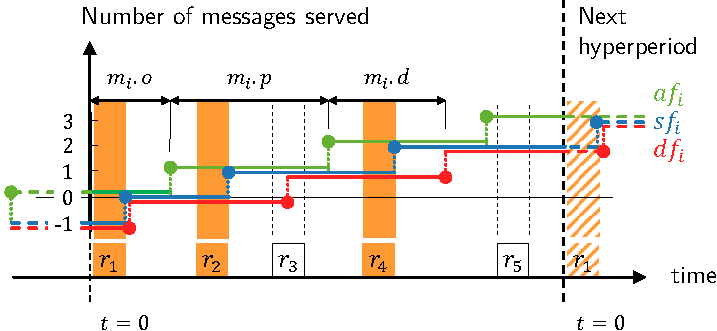
\includegraphics[scale=1]{afdfsf}
\caption{Representation of arrival, demand, and service functions of message $m_i$.
The lower part shows the five round, $r_1$ to $r_5$, scheduled for the hyperperiod.
\capt{%
$m_i$ is allocated a slot in the colored rounds, \ie $r_1$, $r_2$, and $r_4$.
The allocation of $m_i$ to $r_3$ instead of $r_2$ would be invalid, as $r_3$ does not finish before the message deadline, \ie it violates \textbf{(C4.2)}.
However, the allocation of $m_i$ to $r_5$ instead of $r_1$ would be valid and result in $r_0.B_i = 0$.}
}
\label{fig:afdfsf2}
\end{figure}


%-> Introduce integer variables constrained to match the values of \af and \df at time points of interest
\noindent
The arrival and demand functions are step functions. They cannot be used directly in an ILP formulation, however
\begin{flalign}
\label{eq:af=k2}
&\forall \; k \in \mathbb{N}, \quad
&&\af_i(t) = k
	\quad \Leftrightarrow \quad
	0 \, \leq \, t - m_i.o - (k-1)m_i.p \,<\, m_i.p &&\\
&\text{and} %\hspace{30pt}
&&\df_i(t) = k
\label{eq:df=k2}
	\quad \Leftrightarrow \quad
	0 \, < \, t - m_i.o - m_i.d - (k-1)m_i.p \,\leq\, m_i.p &&
\end{flalign}
% We introduce a set of integer variable k^a_{ij} k^d such that
For each message $m_i\in \messageset$ and each round $r_j$, $j \in [1..R_{\mode{}}]$, we introduce two integer variables $k^a_{ij}$ and $k^d_{ij}$ that we constraint to take the values of \af and \df at the time points of interest, \ie $r_j.t$ and $r_j.t + \Tround$ respectively. That is,
\begin{align}
\label{eq:ka2} %\qquad
0 \, \leq \, r_j.t
	&-m_i.o - (k^a_{ij}-1)m_i.p \,<\, m_i.p\\
\label{eq:kd2} %\qquad
0 \, < \, r_j.t
	&+\Tround - m_i.o - m_i.d - (k^d_{ij}-1)m_i.p \,\leq\, m_i.p\\
\notag
\text{Thus,} \hspace{15pt} &\eqref{eq:ka2} \quad \Leftrightarrow  \quad
	 \af_i(r_j.t) = k^a_{ij} \\
\notag
	&\eqref{eq:kd2} \quad \Leftrightarrow \quad
	\df_i(r_j.t + \Tround) = k^d_{ij}
\end{align}

%
%-> Express \sf based on the rounds

\TODO{Here might be the place to say something about the round atomicity...}
Finally, we must express the service function \sf, which counts the number of message instances served \emph{at the end} of each round.
Remember that $r_k.B_s$ denotes the allocation of the $s$-{th} slot of $r_k$.
For any time $t \in \; [ \; r_{j} + \Tround \, ; \,  r_{j+1} + \Tround \; [$, the number of instances of message $m_i$ served is
\begin{align*}
	\sum_{\substack{k = 1}}^{j}
	\sum_{\substack{s = 1}}^{B}
	 \; r_k.B_s
	 \quad s.t. \; B_s = i
\end{align*}

\noindent
It may be that $m.o + m.d > m.p$, resulting in $\df(0)=-1$ (see \eqref{eq:df_def2}), like \eg in \cref{fig:afdfsf2}. This ``means'' that a message released at the each of one hyperperiod will have its deadline in the \emph{next} hyperperiod.
To consider this situation, we introduce, for each message $m_i$, a variable $r_0.B_i$ set to the number of such ``leftover'' message instances at $t=0$.
The system model makes the assumption that $\app.d \leq \app.p$. As $m.p = \app.p$, $m.o \leq m.p$ and $m.d < \app.d$, then $m.o + m.d < 2*m.p$. Thus, there can be only one or zero of such leftover message instances, \ie $r_0.B_i \in \{0\,,\,1\}$.
Finally, for each message $m_i \in \messageset$, and  $t \in \; [ \; r_{j} + \Tround \, ; \,  r_{j+1} + \Tround \; [$,
%
%However, it may be that the last message released during one hyperperiod has its relative deadline in the \emph{next} hyperperiod, thus yielding $df(0)=-1$. It is the case \eg in \cref{fig:afdfsf}. Then, to account for this previously arrived message -- possibly not yet served -- we introduce for each message $m_i$ a variable $r_0.B_i$ set to the value of the service function $sf_i$ of message $m_i$ at $t=0$, that is $0$ or $1$. Thus finally, for each message $m_i \in \messageset$, and  $t \in \; [ \; r_{j} + \Tround \, ; \,  r_{j+1} + \Tround \; [$,
\begin{flalign}
\label{eq:sf_def2}
\sf_i: \; t \;
	&\longmapsto \;
	\sum_{\substack{k = 1 \\[2pt]s.t. \; r_k + \Tround \, < \, t}}^{j}\;\;
	\sum_{\substack{s = 1 \\[2pt]s.t. \; B_s = i}}^{B}
	 r_k.B_s - r_0.B_i
\end{flalign}

\noindent
Ultimately, \textbf{(C4.1)} and \textbf{(C4.2)} can be formulated as ILP constraints using the following four equations:
\begin{flalign}
\notag
\forall\, m_i \in \messageset, \; \forall\, j\in [1..R],
&&&\eqref{eq:ka2}\quad \;	 : \;
	\quad
	0 \, \leq \, r_j.t - m_i.o - (k^a_{ij}-1)*m_i.p \,<\, m_i.p
&&\\
\notag
&&&\eqref{eq:kd2}\quad	\; : \;
	\quad
	0 \, \leq \, r_j.t + \Tround - m_i.o - m_i.d - (k^d_{ij}-1)*m_i.p \,<\, m_i.p
&&\\
&&&\eqref{eq:af_const2}\quad	 \Leftrightarrow
	\quad
	\sum_{k = 1}^j
	\sum_{\substack{s = 1 \\[2pt]s.t. \; B_s = i}}^{B}
	 \; r_k.B_s - r_0.B_i \; \leq\;  k^a_{ij}
&&\\
&&&\eqref{eq:df_const2}\quad	 \Leftrightarrow
	\quad
	\sum_{k = 1}^{j-1}
	\sum_{\substack{s = 1 \\[2pt]s.t. \; B_s = i}}^{B} \; r_k.B_s - r_0.B_i
	\; \geq\;
	k^d_{ij}
&&
\end{flalign}

To implement those constraints in practice, some slight modifications are still required. We use Gurobi to solve the ILP problem. This solver does not allow to model strict inequalities, \ie $A \cdot x  < B$. Therefore, to implement the right-hand side of the constraints \eqref{eq:ka} and \eqref{eq:kd2}, we need to use a ``small'' time constant $mm$.
%
Furthermore,
%
This leads to the following implementation.

\begin{description}
	\item[(C4.1)]Every message must be served after its release time.
\end{description}
\begin{flalign}
&\forall\, m_i\in \messageset, \; \forall\, j\in [1..R_{\mode{}}],
\label{eq:serveAfterArrival}
&	&0  \; \leq \; r_j.t - m_i.o - (k^a_{ij}-1)*m_i.p
		\; \leq \; m_i.p - mm
&		\\
&
&	&\sum_{k = 1}^{j}
	\sum_{\substack{s = 1 \\[2pt]s.t. \; B_s = i}}^{B} \; r_k.B_s - r_0.B_i
	\; \geq\;
	k^d_{ij}
&
\intertext{%
\begin{description}
	\item[(C4.2)]Every message must be served before its deadline.
\end{description}
}
&\forall\, m_i\in \messageset, \; \forall\, j\in [1..R_{\mode{}}],
&	&mm  \; \leq \; r_j.t + \Tround - m_i.o - m_i.d - (k^d_{ij}-1)*m_i.p
		\; \leq \; m_i.p
&		\\
&
&	&\sum_{k = 1}^{j-1}
	\sum_{\substack{s = 1 \\[2pt]s.t. \; B_s = i}}^{B} \; r_k.B_s - r_0.B_i
	\; \geq\;
	k^d_{ij}
&
\end{flalign}

Finally, the formulation of the last two constraints -- \textbf{(C4.3)} and \textbf{(C4.4)} -- is rather straightforward.

\begin{description}
	\item[(C4.3)]A round cannot be allocated more messages than the number of slots available in one round.
\end{description}
%
\begin{align*}
\text{Satisfied by construction.}
\end{align*}


\begin{description}
	\item[(C4.4)] Within one hyperperiod, the same number of messages are released and served.
\end{description}
\begin{flalign}
&\forall\, m_i\in \messageset,
&
	&\sum_{k = 1}^{R_{\mode{}}}
	\sum_{\substack{s = 1 \\[2pt]s.t. \; B_s = i}}^{B} \; r_k.B_s
	\; = \; LCM/m_i.p
&&
\end{flalign}

\subsection*{Objective function}

To obtain a valid schedule, the ILP solver does not \emph{need} to optimize any objective function. The primer objective is to minimize of the number of rounds $R_{\mode{}}$ used in the schedule, which is achieved by incrementally increasing the number of rounds (see Algorithm~\ref{alg:outerlayer}) until a valid schedule is found.

However, from the application perspective, it is of importance to \emph{minimize the end-to-end latency} of concurrently running applications. Therefore, we formulate as an objective function, denoted \obj, the sum of all application latency, which we want to minimize. If we denote the latency of application \app by $\app.\delta$ and the latency of the chain $\app.c$ by $\app.c.\delta$,
\begin{align}
\intertext{%
$	\forall\, \app, \;
	\forall\, \app.c \in \app.\predG, \;
		\tau_{\first} = \app.c(\,\first\,), \;
		\tau_{\last} = \app.c(\,\last\,), \;
		C = |\app.c|, $}
\app.c.\delta \; & = \;
%	\max
%		\left(
			\tau_{\last}.o + \tau_{\last}.e - \tau_{\first}.o + \sum_{j=1}^{C-1} \app.p*				\sigma_{i,j}
%		\right)
\\
 \app.\delta \; &= \;
	\max_{\app.c \,\in\, \app.\predG}
		\left(
			\;
			\app.c.\delta
			\;
		\right)
\intertext{%
And finally,}
\obj \; &= \; \sum_{\app \,\in\, \text{mode }\mode{}} \;
	\app.\delta
\end{align}


\begin{table}[h]
\centering
\small
\caption{Complete list of variables used in the ILP formulation.}
\label{tab:ILPvar}
\input{\ChapPath/Tables/table_ILPvar.txt}
\end{table}

  % \newpage
  % % !TEX root = ../00_thesis.tex

\section{Appendix B}
% \subsection*{Additional constraints for the multi-mode schedule synthesis problem}
\label{appendix:multi_mode}

In this appendix, we present how are practically implemented the constraints ensuring that
\begin{itemize}

	\item Schedules in the multi-mode case are compatible, \ie the inheritance constraints formulated in Theorem~\ref{thm:minVirtLegacy} (\cref{sec:multi_mode}) are respected

	\item Running applications can seamlessly switch between modes, \ie there is no risk of missed deadline due to a mode change, as described in \cref{sec:modeChanges}.

\end{itemize}
Finally, we conclude with a short comment on how to implement context-specific requirements in the schedule synthesis problem.

\vspace{10pt}
\fakepar{Compatible schedules}
Let us consider the schedule synthesis of mode \mode{j} where applications \app and \appB have been scheduled in higher-priority mode \mode{i}, such that
\begin{itemize}

	\item $\exists \; \app \in \legApp{j}$

	\item $\exists \; \appX \in \freeApp{j} \, , \; \appB \in \minvirtlegApp{j}{\appX}$

\end{itemize}
We denote with a superscript $^k$ a schedule value computed in mode \mode{k}, \eg $m^j.o$ is the offset of message $m$ computed in mode \mode{j}.

%legacy app: fix everything.
\app is a legacy application for mode \mode{j}. Its schedule must be reserved, which is realized simply as follows
\begin{flalign}
&\forall \; (\tau, m) \in \app.c,
&	\tau^{j}.o \; &= \; \tau^i.o
&&\\
&
&	m^i.o \; &= \; m^j.o
&&\\
&
&	m^i.d \; &= \; m^j.d
&&
\end{flalign}

%virtual legacy app: use
\appB is a virtual legacy application for application \appX. As a result, the scheduling ``space'' of the tasks of \appB must be reserved, to guarantee that the tasks of \appX will not overlap with \appB. This is achieved by adding constraints similar to those enforcing (C3), guaranteeing the validity of the task mappings (see the previous Appendix)
%
\begin{align}
\intertext{%
$	\forall\,
		\tau_\appB \in \appB.c	, \,
		\tau_\appX \in \appX.c  , \;
		\; E_\appB == E_\appX, \;
	\forall\, k_\appB \in [1..LCM/\tau_\appB.p], \; \forall\, k_\appX \in [1..LCM/\tau_\appX.p]$}
	\tau_\appB.o + \tau_\appB.e + \tau_\appB.p*k_\appB
	&\; \leq \; \tau_\appX.o + \tau_\appX.p*k_\appX \\
\texttt{or} \quad
	\tau_\appX.o + \tau_\appX.e + \tau_\appX.p*k_\appX
	&\; \leq \; \tau_\appB.o + \tau_\appB.p*k_\appB
\end{align}
%
Similarly, the \; \texttt{or} \; condition is realized using a ``big'' time constant $M$ and boolean variables.
%
\begin{align}
\tau_\appB.o + \tau_\appB.e + \tau_\appB.p*k_\appB
	&\; \leq \; \tau_\appX.o + \tau_\appX.p*k_\appX
		+ M * (1 - \lambda_{\appB,\appX}^{k_\appB,k_\appX})\\
\tau_\appX.o + \tau_\appX.e + \tau_\appX.p*k_\appX
	&\; \leq \; \tau_\appB.o + \tau_\appB.p*k_\appB
		+ M * \lambda_{\appB,\appX}^{k_\appB,k_\appX}
\end{align}


\vspace{10pt}
\fakepar{Seamless mode switch}
%message served and released in the same hyperperiod
In order to prevent the risk of missed deadline due to a mode change, we described in \cref{sec:modeChanges} a simple procedure to execute mode change requests.
\begin{enumerate}

	\item All messages must be released and served within the same hyperperiod.
	\label{rule1}

	\item The starting time \tjstart of mode \modej is set to the end of the first hyperperiod of \modei after which the execution of all applications $\app \in \Sij$ has been completed.

\end{enumerate}
%
The second rule depends on the embedded software, it is independent of the schedule synthesis.
To enforce the first rule however, additional constraints must be formulated. As discussed at the end of \cref{sec:single_mode} and illustrated in \cref{fig:openboxoptions}, the rounds schedule may be such that some messages are released in one of the mode's hyperperiod, but served only in the next hyperperiod, see~\cref{subfig:case2}.
\TODO{Now the only case presented in df(0) = -1, adapt the text}

For applications scheduled in only one mode, this is no problem. Indeed, for every mode changed, they are either starting, terminating, or not involved, which cannot lead to a deadline miss.
For the other applications, \ie scheduled in more than one mode, we enforce rule (\ref{rule1}) by setting the parameters $r_o.B_i$ in the definition of the service function $sf_i$~(see \eqref{eq:sf_def}).
For any application \app scheduled in more than one mode,
%
\begin{flalign}
&
\forall \, m_i \in \app.c,
&&r_o.B_i \; = \; 0
&&
\end{flalign}
%



\vspace{5pt}
\fakepar{Context-specific requirements}
The scheduling framework proposed in this work is very flexible thanks to the use of an ILP formulation to synthesize the schedules.
We described in the Appendices a set of constraints for this ILP formulation that solves our initial problem, as stated in \cref{sec:model}.
Then, additional constraints can be added to the formulation, to capture context-specific requirements. We give thereafter some examples of practically-relevant constraints.

\vspace{5pt}
\begin{description}

	\item[Tasks $\tau_1$ and $\tau_2$ must start simultaneously]
	\begin{equation}
	\tau_1.o \; = \;  \tau_2.o
	\end{equation}

	\item[The time difference between $\tau_1$ finishing and $\tau_2$ starting is bounded by $D$]
	\begin{equation}
	\tau_2.o - ( \, \tau_1.o + \tau_1.e \, ) \; \leq \; D
	\end{equation}

	\item[Messages $m_1$ and $m_2$ must be allocated to the same rounds]
	\begin{flalign}
	&\forall\, j\in [1..R],
	&&r_j.B_1 \; = \; r_j.B_2 \qquad
	&&
	\end{flalign}

\end{description}

  % \newpage
  % !TEX root = ../00_thesis.tex

\section{System Configuration -- Scheduler Evaluation}
\label{append:inheritance_eval}

This appendix details the system configuration used for the performance evaluation of \TTW's scheduler~(\cref{sec:ttw_evaluation_sched}).
The configuration consists of 15 different applications involving 45 tasks and 30 messages, executing in 5 different modes~(\cref{table:modes}).
All applications are considered persistent, and the precedence graphs always contain a single chain.
The tasks are mapped to 13 different nodes~(\cref{table:mapping}), with a WCET set to 1\ms.
The mode graph is shown in~\cref{fig:modeGraph_eval}.
% All other inputs are set as reported in \cref{tab:ILPvar}.


\begin{table}[b]
  \centering
  \caption{Task mapping for \TTW's scheduler evaluation~(\cref{sec:ttw_evaluation_sched}).}
  \label{table:mapping}
  {\smaller \input{\TablePath/mapping.csv}}
\end{table}

\begin{table}[b]
  \centering
  \caption{System configuration for \TTW's scheduler evaluation~(\cref{sec:ttw_evaluation_sched}).}
  \label{table:modes}
  {\smaller \input{\TablePath/modes.csv}}
\end{table}

\end{subappendices}
